\chapter{Data Analysis}
\label{cha:data_analysis}
As mentioned earlier, despite the fast helicity flipping and extensive effort to maintain
the electron beam under identical conditions during opposite helicity states, 
achieving this goal completely is practically impossible. Various noises are 
inevitably generated in different parts of the accelerator. While these noises
are generally small, they can still have a significant impact on our measurements
if not properly addressed.

We used the same methods for processing both the PREX-II and CREX data sets. 
Therefore, we will discuss only CREX data here, anything that is different in PREX-II will be
highlighted.

\begin{table}
    \centering
% with cut ErrorFlag&0xda7e6bff == 0 and minirun_size >= 4500
    \begin{tabular}{c | c}
	\hline
	Number of Good Slugs	    & 121   \\
	Number of Good Runs	    & 1384  \\
	Number of Good Miniruns	    & 8525  \\
	Number of Good Quadruplets  & 86832046  \\
	\hline
	Charge Asymmetry    & $\sim 100$~ppb	\\
	Position Difference & $\sim 10$~nm  \\
	Angle Difference    & $\sim 1$~nrad \\
	Energy Difference   & $\sim 10$~ppb \\
	\hline	    
	Raw Asymmetry	    & $2087$~ppm    \\
	Regressed Asymmetry & $2090$~ppm    \\
	\hline
    \end{tabular}
    \caption{CREX data statistics.}
\end{table}

% \begin{table}
%     \centering
%     \begin{tabular}{c | c c c}
% 	\hline
% 	Variable    & Regression    & Dithering	    & Lagrangian    \\
% 	\hline
% 	Slope	\\
% 	Correction (ppm)  \\
% 	\hline
%     \end{tabular}
% \end{table}

\begin{comment}
    % https://prex.jlab.org/DocDB/0000/000009/001/riordan_err_recommend-3.pdf
    \begin{itemize}
	\item (design) PREX-II statistical width: $\sim 120\ ppm @30Hz$
	\item (design) BCM resolution: $40\ ppm$
	\item (measured) 1 MHz BCM electronics: $\sim 25\ ppm @30 Hz, 20\ \mu A$
	\item charge and position jitter
	    $$ A_Q: 100-300\ ppm \quad \Delta x: 5-25\ \mu m$$
    \end{itemize}
\end{comment}

%%%%%%%%%%%%%%%%%%%%%%%%%%%%%%%%%%%%%%%%%%%%%%%%%%%%%%%%%%%%%%%%%%%%%%%%
\section{Raw Data}
CREX started commissioning around December 2019, the first good run was taken on 
December 12th. Six slugs (slug 100 - 105. See discussion below for the definition of slug) 
were collected before the Christmas break. Data
taking resumed after the break and continued until January 18th, 2020 when the first \Ca 
target was damaged. It took five days to prepare a new target.
Following the target replacement, the experiment proceeded smoothly. 
From February 10th to February 12th, we conducted a two-day measurement of the 
transverse asymmetry (AT). We have collected slightly more than half of the desired
charge when Covid-19 hit, which led to the shutdown of the lab at the end of March 2020. 
Fortunately, the lab reopened four months later, providing us with an opportunity
to resume electron bombardment for another month. 
The data taking phase of the experiment concluded on September 18th, 2020. In total, a charge of 480 C was collected, with 390 C considered to be of good quality.

The data set is clearly separated into three distinct periods: 
before the AT, after the AT but before the Covid, and after the Covid, in chronological order. 
A more reasonable split is to separate them based on the Wien-flip states, 
whose result aligns closely with the chronological divisions.

\begin{figure}[!h]
    \begin{tikzpicture}
	\begin{scope}
	    \node[anchor=south west, inner sep=0] (image) at (0, 0)
	    {   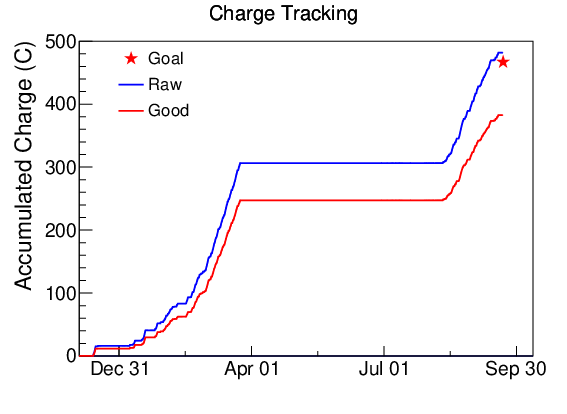
\includegraphics[width=0.45\linewidth]{charge_vs_time}
		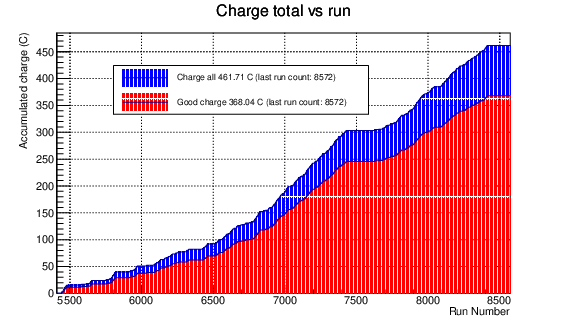
\includegraphics[width=0.55\linewidth]{charge_vs_run} };
	    \begin{scope}[x={(image.south east)},y={(image.north west)}]
		\node [Violet] at (0.27, 0.8) {Covid-shutdown};
		\draw [-stealth, Violet, line width=1pt] (0.28, 0.75) -- (0.28, 0.6);
		\node [Violet] at (0.14, 0.65) {AT};
		\draw [-stealth, Violet, line width=1pt] (0.14, 0.61) -- (0.14, 0.3);
	    \end{scope}
	\end{scope}
    \end{tikzpicture}
    \caption[charge accumulation]
    {Charge accumulation versus time (left) and the run number (right). The
    extended plateau in the left plot corresponds to period of the the Covid-19 shutdown, 
    which is shown around run 7500 in the right plot. One sees that data taking 
    is most efficient after the AT and before the Covid. The last month (after the Covid) 
    shows reasonably efficient data taking, while the first two months of data
    collecion are less efficient due to various hardware problems encountered.}
\end{figure}

In total, CREX collected 1451 production runs. Out of these, 1386 were identified as `Good'
and were used for final analysis. The good runs consists of 1362 both arms runs,
6 left arm runs and 18 right arm runs. Each good production run lasts about 1~hour
and collects about 0.3~C with a charge efficiency of 80\%.
\begin{figure}[!h]
    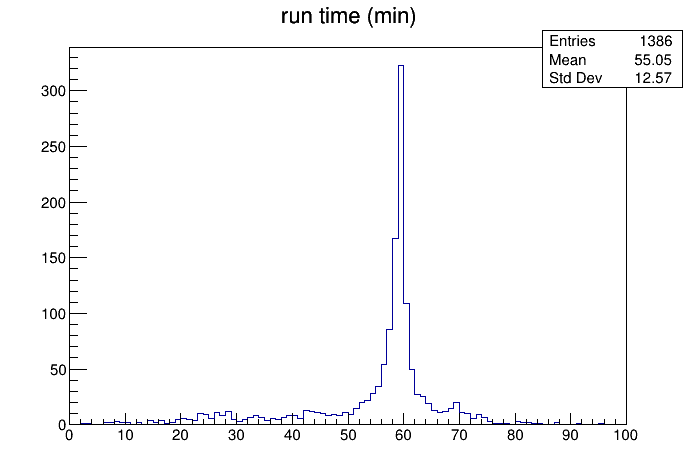
\includegraphics[width=0.32\linewidth]{crex_run_time}
    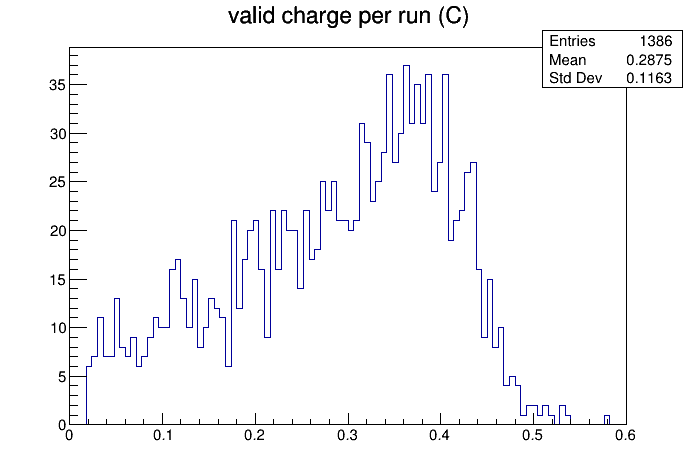
\includegraphics[width=0.32\linewidth]{crex_run_charge}
    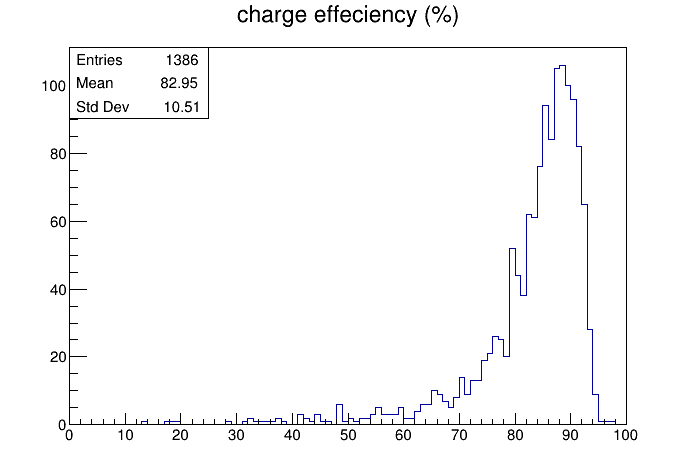
\includegraphics[width=0.32\linewidth]{crex_run_charge_efficiency}
    \caption{Runtime and charge statistics of CREX runs (\texttt{ErrorFlag == 0}).}
\end{figure}

Although electrons arrive in bunches, with a buch frequency of 499~MHz, this frequency
is much higher than the helicity flip frequency of 120~Hz. Consequently, 
the electron beams can be regarded as continuous. In each helicity window, all 
scattered electrons are integrated into a single readout (event).
Every four continuous helicity events are grouped into one quadruplet
(in case of the 240~Hz flipping frequency in PREX-II, every eight helicity events 
form one octuplet).
To mitigate the impact of 60~Hz line power noise, the PV asymmetry is calculated based on helicity quadruplets (or octuplets in the case of a 240 Hz flipping frequency). Every four continuous helicity events form a quadruplet (or every eight events form an octuplet in PREX-II).
The frequency of the helicity quadruplets is 30~Hz, as shown in Fig.~\ref{fig:helicity_pattern}. This choice of frequency allows for effective cancellation of the 60 Hz line power noise. Throughout the CREX experiment, approximately 87 million good helicity quadruplets were collected.
\begin{figure}[!h]
    \centering
    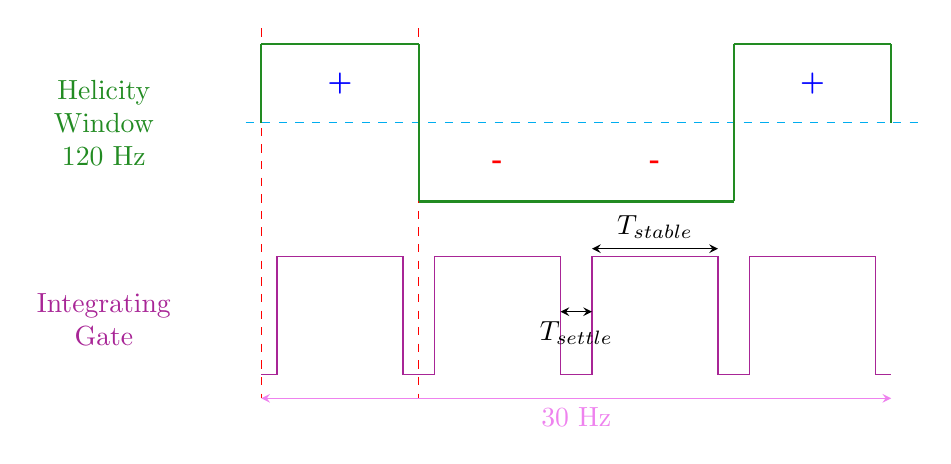
\begin{tikzpicture}[xscale=2]
	\tikzstyle{message} = [align = center]
	\draw[dashed, cyan] (-0.1, 0) -- (4.2, 0);
	\foreach \x in {0, 1}
	{ \draw[dashed, red] (\x, 1.2) -- (\x, -3.5); }
	\foreach \x in {0, 4}
	{ \draw[thick, ForestGreen] (\x, 0) -- (\x, 1); }
	\foreach \x in {1, 3}
	{ \draw[thick, ForestGreen] (\x, -1) -- (\x, 1); }
	\foreach \x in {0, 3}
	{ 
	    \draw[thick, ForestGreen] (\x, 1) -- +(1, 0); 
	    \node[blue] at (\x+0.5, 0.5) {\textbf{+}};
	}
	\foreach \x in {1, 2}
	{ 
	    \draw[thick, ForestGreen] (\x, -1) -- +(1, 0); 
	    \node[red] at (\x+0.5, -0.5) {\textbf{-}};
	}
	\node[message, ForestGreen, very thick] at (-1, 0) {Helicity \\  Window \\ 120 Hz};

	\foreach \x in {0, ..., 3}
	{
	    \draw[Mulberry] (\x, -3.2) -- ++(0.1, 0) -- ++(0, 1.5) -- ++(0.8, 0) 
	    -- ++(0, -1.5) -- ++(0.1, 0);
	}
	\draw[stealth-stealth, black] (2.1, -1.6) -- node[above] {$T_{\text{stable}}$}+(0.8, 0) ;
	\draw[stealth-stealth, black] (1.9, -2.4) -- node[below] {$T_{\text{settle}}$}+(0.2, 0) ;
	\draw[stealth-stealth, Violet] (0, -3.5) -- node[below] {30 Hz} +(4, 0);
	\node[message, Mulberry, very thick] at (-1, -2.5) {Integrating \\ Gate};
    \end{tikzpicture}
    \caption[Helicity pattern]
    {Schematic plot of the helicity pattern. In CREX, $T_{\text{settle}} = 90\ \mu$s, 
    which allows the PC to stabilize after a voltage polarity flipping, avoiding 
    any cross-effect from the previous helicity state. The corresponding deputy factor 
    is 98.92\%.}
    \label{fig:helicity_pattern}
\end{figure}

\begin{figure}[!h]
    \centering
    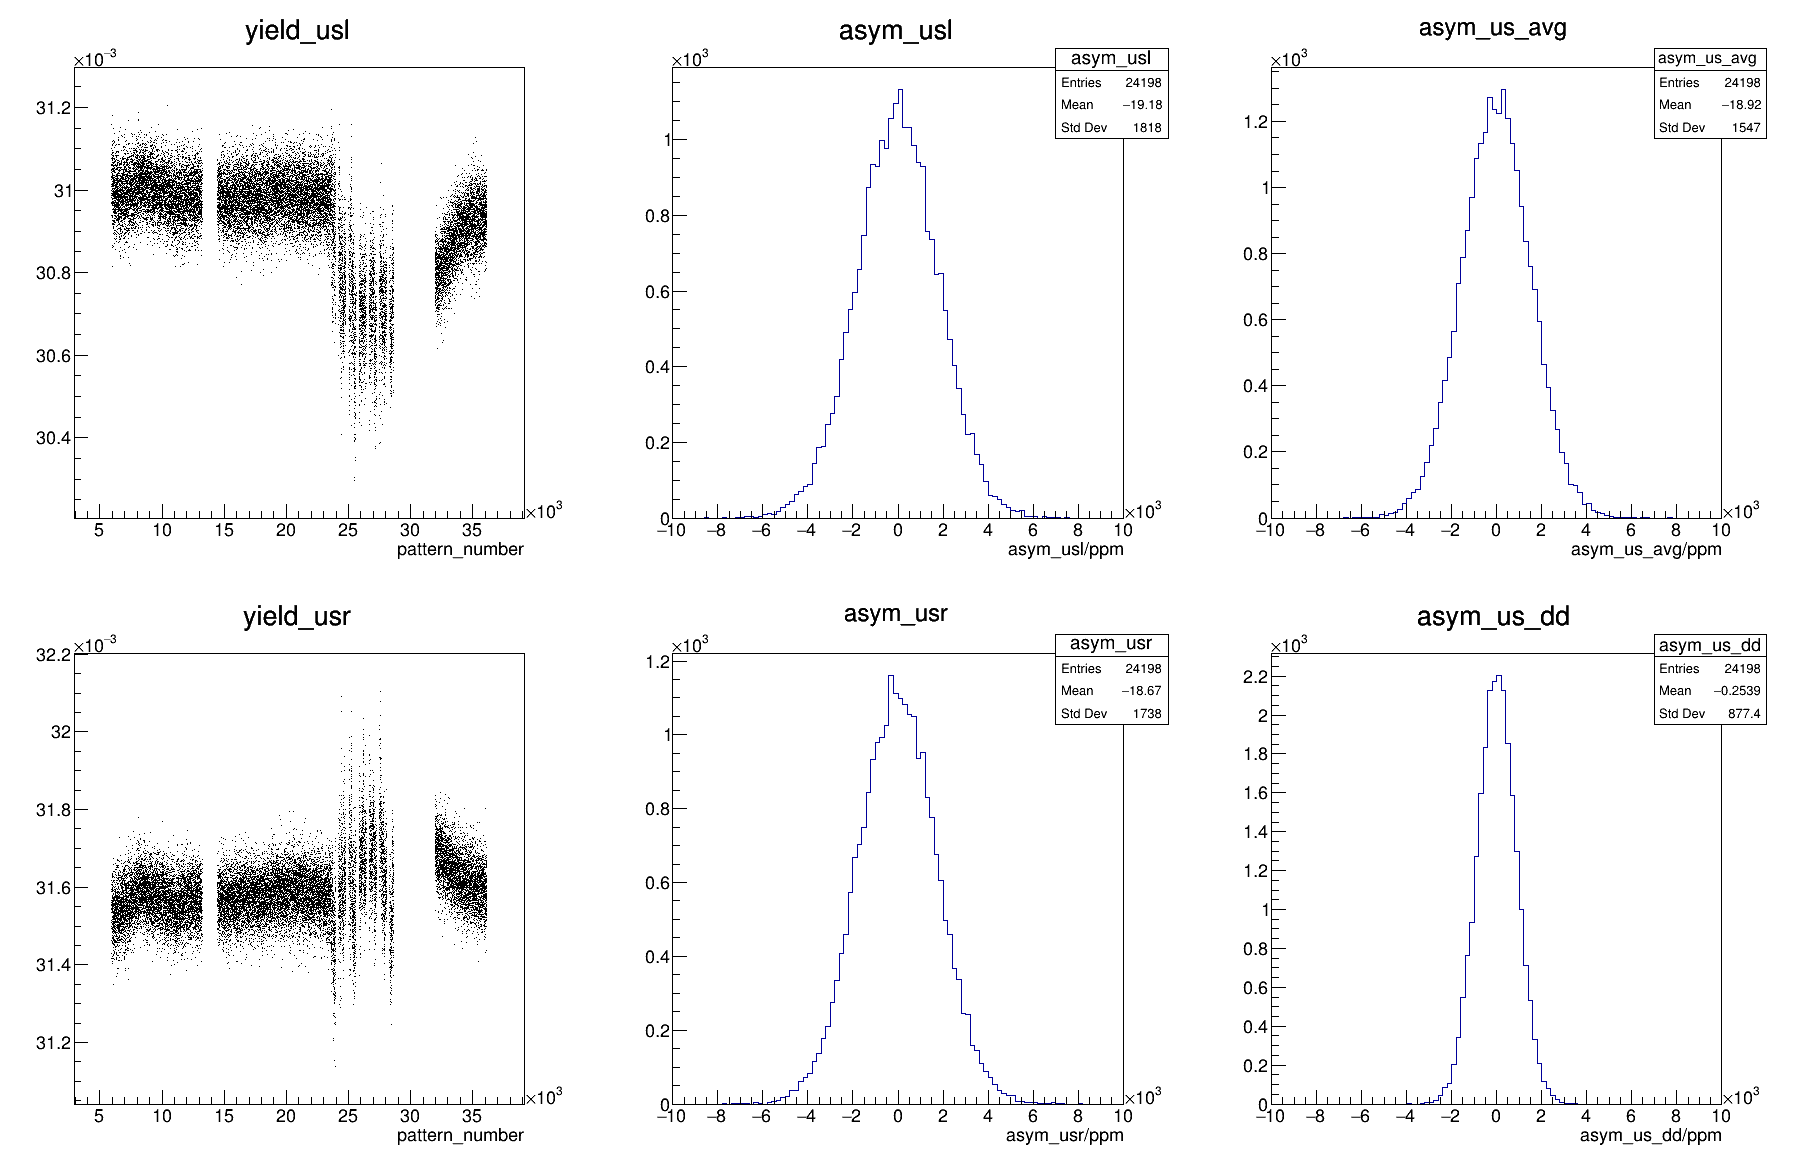
\includegraphics[width=\linewidth]{run_6600_maindet}
    \caption[A `run' plot: detector yield and asymmetry distribution in run 6600]
    {A `run' plot: detector yield and asymmetry distribution in run 6600, 
    selected with \texttt{ErrorFlag == 0}. The observed shift in the second half of the 
    yield plot can be attributed to fluctuations in the beam position and angle. 
    The right two plots display the average and difference of the asymmetry betwen 
    the LHRS and RHRS. 
    Ideally, the difference should be zero and the average is what we want to measure.
    }
\end{figure}

To account for the rapidly changing beam conditions, each run is divided into
multiple miniruns. Calculating the detector slope, which is the detector's 
response to beam fluctuations, over a 60~mins time scale is inappropriate.
It is more appropriate to do the calculation over the duration of a minirun
since the beam conditions, and consequently the slope value, tend to be
more stable within a shorter time period.  

Every minirun contains 9000 good helicity quadruplets, corresponding to about 5~mins
of data collection. The last minirun in each run contains the remaining
quadruplets that cannot be divided into two separate miniruns. 

Miniruns with a number of samples less than half of the standard (4500) are discarded.
In total, CREX has 8543 miniruns from 1386 good runs. Among these, 2 miniruns are discarded
due to their small sample size, while 16 miniruns are discarded due to noisy beam conditions 
or large beam shifts that were not caught in the previous two analysis campaigns (respin). 
To avoid another respin, these miniruns are simply removed. % which counts ??? C.
The discarded miniruns are listed out in Table~\ref{tab:short_miniruns} and \ref{tab:bad_miniruns}.
\begin{table}[!h]
    \centering
    \begin{tabular}{c c c}
	\hline
	run & minirun	& number of samples \\
	\hline
	% 5972	& 0 & 4385  \\
	% 6691	& 0 & 4080  \\
	7720	& 0 & 4352  \\
	8082	& 0 & 4391  \\
	\hline
    \end{tabular}
    \caption{Two miniruns that have too small good samples (with cut \texttt{ErrorFlag == 0}).}
    \label{tab:short_miniruns}
\end{table}
\begin{table}[!h]
% http://ace.phys.virginia.edu/HAPPEX/4606
    \centering
    \begin{tabular}{c c | c c}
	\hline
	run & minirun	& run	& minirun   \\
	\hline
	6564	& 4	& 7211	& 4 \\
	6567	& 2, 4	& 7889	& 0 \\
	6571	& 3, 4	& 7942	& 5 \\
	6593	& 2	& 8036	& 2 \\
	6983	& 8	& 8240	& 1 \\
	7149	& 6	& 8549	& 0, 1, 4   \\
	\hline
    \end{tabular}
    \caption{List of Miniruns that had larger asymmetry outliers and therefore
    are removed.}
    \label{tab:bad_miniruns}
\end{table}
\begin{figure}[!h]
    \centering
    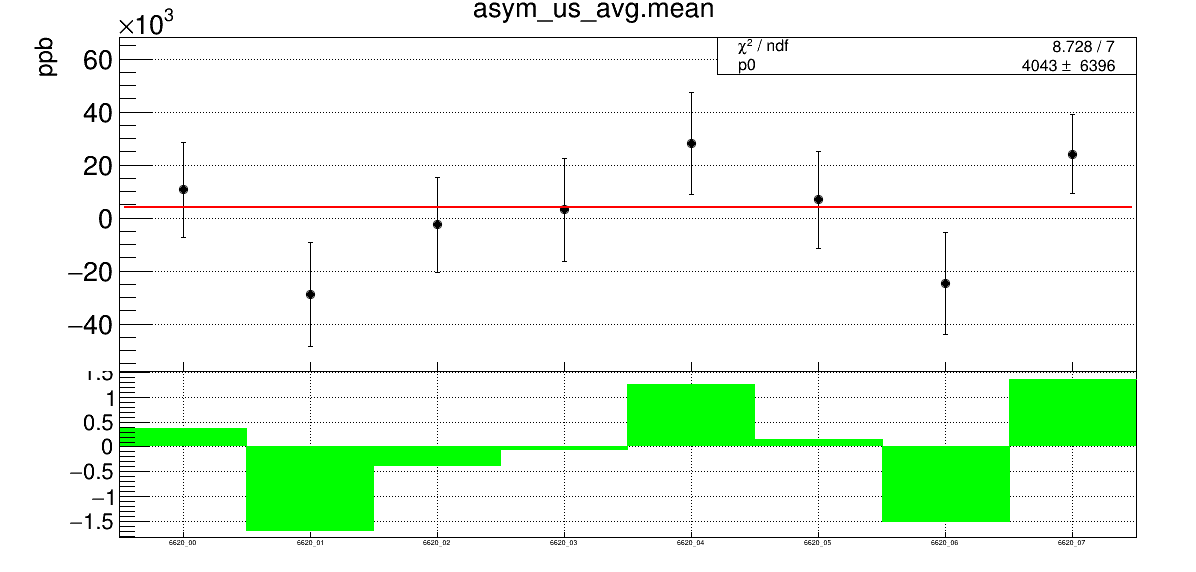
\includegraphics[width=\linewidth]{run_6620_mini_asym_us_avg.mean}
    \caption[A minirun plot]
    {A `minirun' plot: mean values of asym\_us\_avg of each minirun in 
    run 6620 (\texttt{ErrorFlag == 0}).
    The red line is a zero-order polynomial fit and the bottom histogram is
    the ratio of the deviation to the mean fit value with respect to each point's uncertainty.
    }
\end{figure}

Runs are grouped into slugs. A slug is defined as the collection of runs between two
changes of the IHWP. Under stable beam conditions, we could collect three slugs per day. 
Therefore, each slug corresponds to about 8~hours of data collection, although
this duration may be extended in case of any issues. In total, CREX collects
124 slugs. After the data cleaning and combining slugs to remove those with only one run, 
121 slugs are retained.
% slug 100 - 223
% slug 105, 117 and 123 are removed
\begin{figure}[!h]
    \centering
    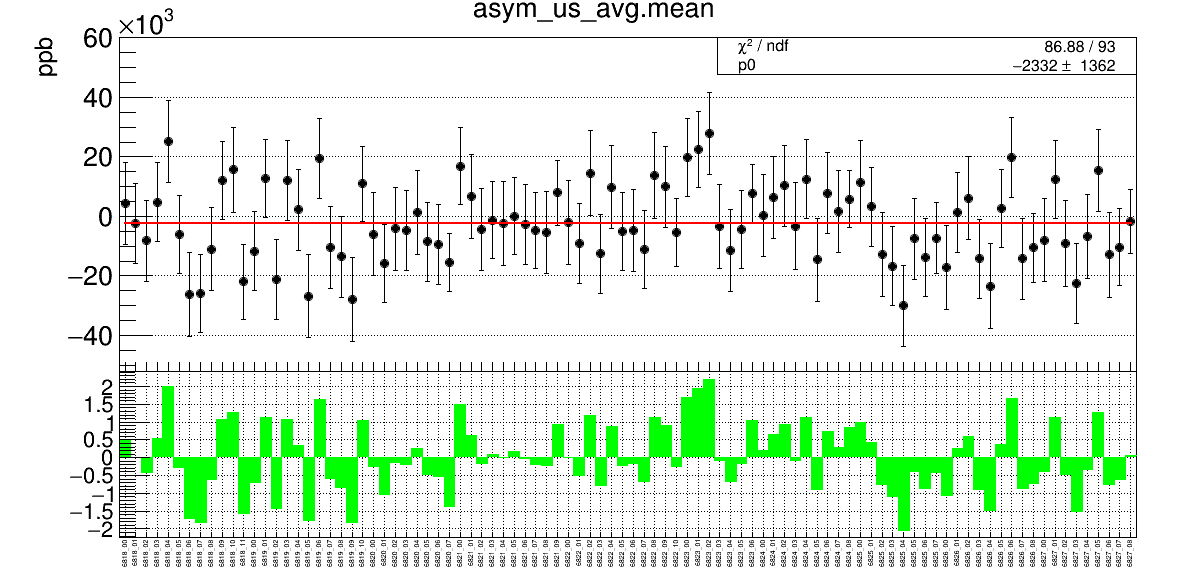
\includegraphics[width=\linewidth]{slug_150_asym_us_avg.mean}
    \caption[A slug plot]
    {A slug plot: minirun-wise distribution of asym\_us\_avg in slug 150 
    (\texttt{ErrorFlag == 0}).}
\end{figure}

Finally, slugs are further divided into periods based on their Wien flip states. 
As mentioned earlier, there are three distinct periods.
\begin{table}[!h]
    \centering
    \begin{tabular}{c | c}
	\hline
	Wien-flip   & slugs \\
	\hline
	Right	& 100-137   \\
	Left	& 138-185   \\
	Right	& 186-223   \\
	\hline
    \end{tabular}
    \caption{Wien-flip separation in terms of slugs.}
\end{table}

%%%%%%%%%%%%%%%%%%%%%%%%%%%%%%%%%%%%%%%%%%%%%%%%
\subsection{Cut}
A loose cut is applied at the event level to maximize the selection of good events.
During the data taking process, the JAPAN monitors various aspects, such as 
hardware failures, beam stability, helicity information and others. These parameters
are checked against a total of 23 criteria. Based on the results of these checks,
an error code (ErrorFlag) is assigned to each event. The error code is obtained 
by performing a bitwise OR operation on the results of all the checks. 
Events that pass all 23 checks will have a null error code (ErrorFlag == 0). 

The various hardware failure checks are designed to detect issues related to the
ADC readout in the detectors and monitors. These checks ensure that the recorded
data does not contain saturated or null values. These checks help to identify the problematic
hardware channels in case of any hardware failures.

The beam stability level checks monitor the beam conditions by analyzing the
mean and RMS values of detector and monitor readouts. These checks compare the 
readout values to user-defined upper and lower limits to identify outliers. 
Additionally, for some ADC channels, there are cuts based on the RMS values 
calculated over a moving time window of 200 (configurable) % prex_ring_stability.xxxx.conf
consecutive events, if the RMS value exceeds a certain threshold,
all events within that time window fail the RMS check. 
Furthermore, the burplevel check compares the current event readout with the average
value of the previous 10 (configurable) events. If the difference between the 
current event and the average value exceeds a specific threshold (burplevel cut),
the event fails the burplevel check. 

One example of such stability cuts is the beam current cut. In the event of a
beam trip caused by accidents or other factors, the beam intensity drops and 
then recovers quickly. During this falling and rising process, the beam stability
is typically compromised. To ensure the quality of the data, a requirement is imposed that the event beam current should be larger than the stable beam current minus $30\ \mu$A ($15\ \mu$A in PREX-II).

By implementing these beam stability level checks, we can make sure that the collected
data meets quality standards.
\begin{figure}[!h]
    \centering
    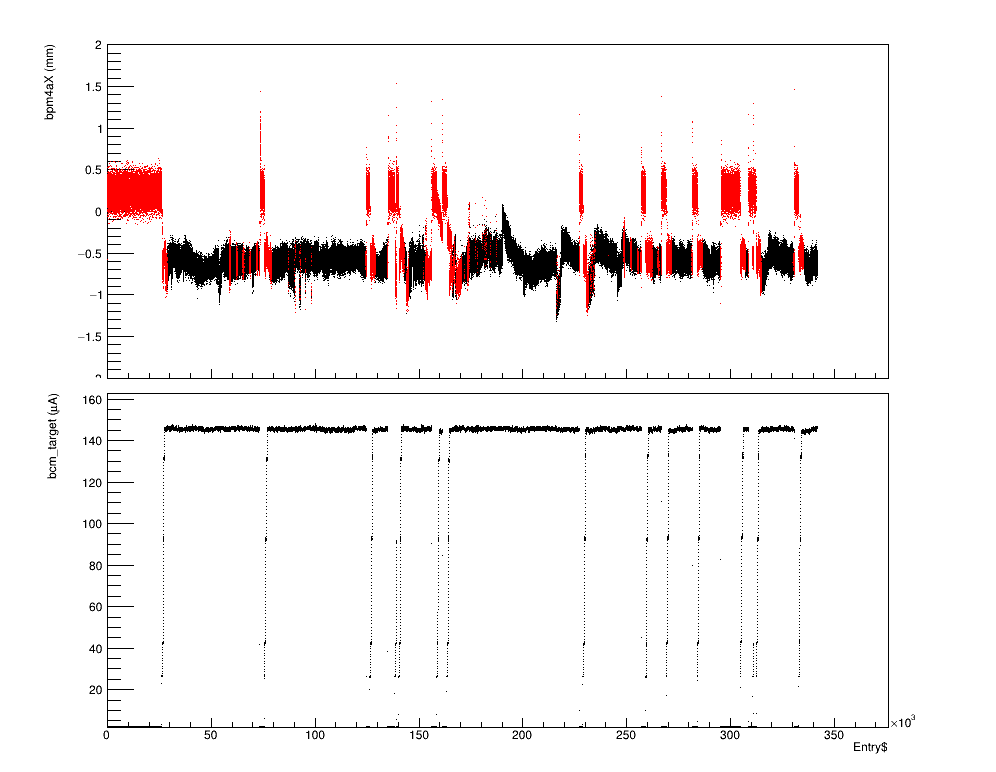
\includegraphics[width=\linewidth]{8019_bpm4aX}
    % 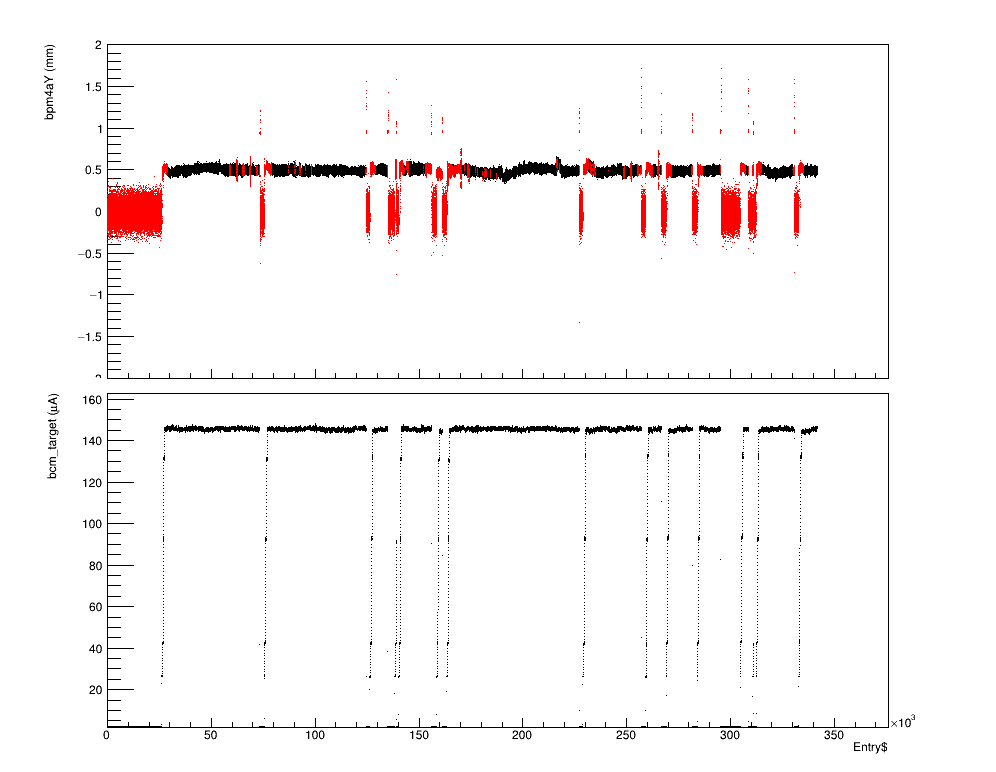
\includegraphics[scale=0.28]{8019_bpm4aY}
    \caption[BPM4aX distribution in run 8019]
    {BPM4aX distribution (top) in run 8019, the bottom plot is the corresponding
    beam current distribution. Black points are good events (\texttt{ErrorFlag == 0}) 
    and red points are bad ones (\texttt{ErrorFlag != 0}). 
    One can clearly see that all beam trips and most beam jitters are recognized 
    by our stability checks.}
\end{figure}

In addition to these checks, we have an analysis shift worker to check monitor/detector 
yields and their differences/asymmetries for each run. If the shift worker observes large beam excursions, drifts, or any other irregularities in the monitor/detector yields or their differences/asymmetries, additional cuts can be applied. These cuts are specific to each run and are added one by one as needed. 

During both the online and the offline analyser, we used cut \verb|ErrorFlag == 0|
to select good quadruplets. This cut excludes all beam modulation events. However, 
some beam modulation events are actually usable for our asymmetry analysis and were
included in the final published result. These modulation events counts for about 
5\% of the CREX data set.
To be consistent with the published result, all following plots are produced with the cut 
\verb|ErrorFlag&0xda7e6bff == 0| if not mentioned otherwise. 
% http://ace.phys.virginia.edu/HAPPEX/4611

%%%%%%%%%%%%%%%%%%%%%%%%%%%%%%%%%%%%%%%%%%%%%%%%
\subsection{Beam Conditions}
As explained before, maintaining consistent experimental conditions is crucial for accurately measuring small asymmetry values. Among these conditions, the most challenging one to control is the beam condition. Fluctuations in any component along the lengthy accelerator line can lead to changes in the beam condition, potentially introducing noise asymmetry into our measurements.

Despite these challenges, the dedicated CEBAF staff has made significant efforts to provide us with excellent beams that exhibit minimal differences between different helicity windows.

%%%%%%%%%%%%%%%%%%%%%%%%
\subsubsection{Beam Current}
The raw asymmetry is normalized to the beam current in order to account for variations in beam current between runs and within a single run, where the beam currents may differ slightly between helicity windows. The normalized raw asymmetry is:
\begin{equation}
    \CA_{\text{raw}} = \frac{(D/I)^+ - (D/I)^-}{(D/I)^+ + (D/I)^-}
	\approx \frac{D^+ - D^-}{D^+ + D^-} - \frac{I^+ - I^-}{I^+ + I^-}
	= \CA_D - \CA_I
\end{equation}
where D represents the detector readout.

This equation demonstrates that the charge asymmetry contributes to the raw asymmetry directly.
Therefore, it is desirable to minimize the charge asymmetry, which is achieved 
through the charge feedback system. The charge asymmetry is typically on the order
of hundreds of ppb, as shown in Fig.~\ref{fig:crex_bcm_target}.
From this figure, one can also observe 
that period 2 has relatively more stable beam conditions compared to the other two periods.
\begin{figure}[H]
    \centering
    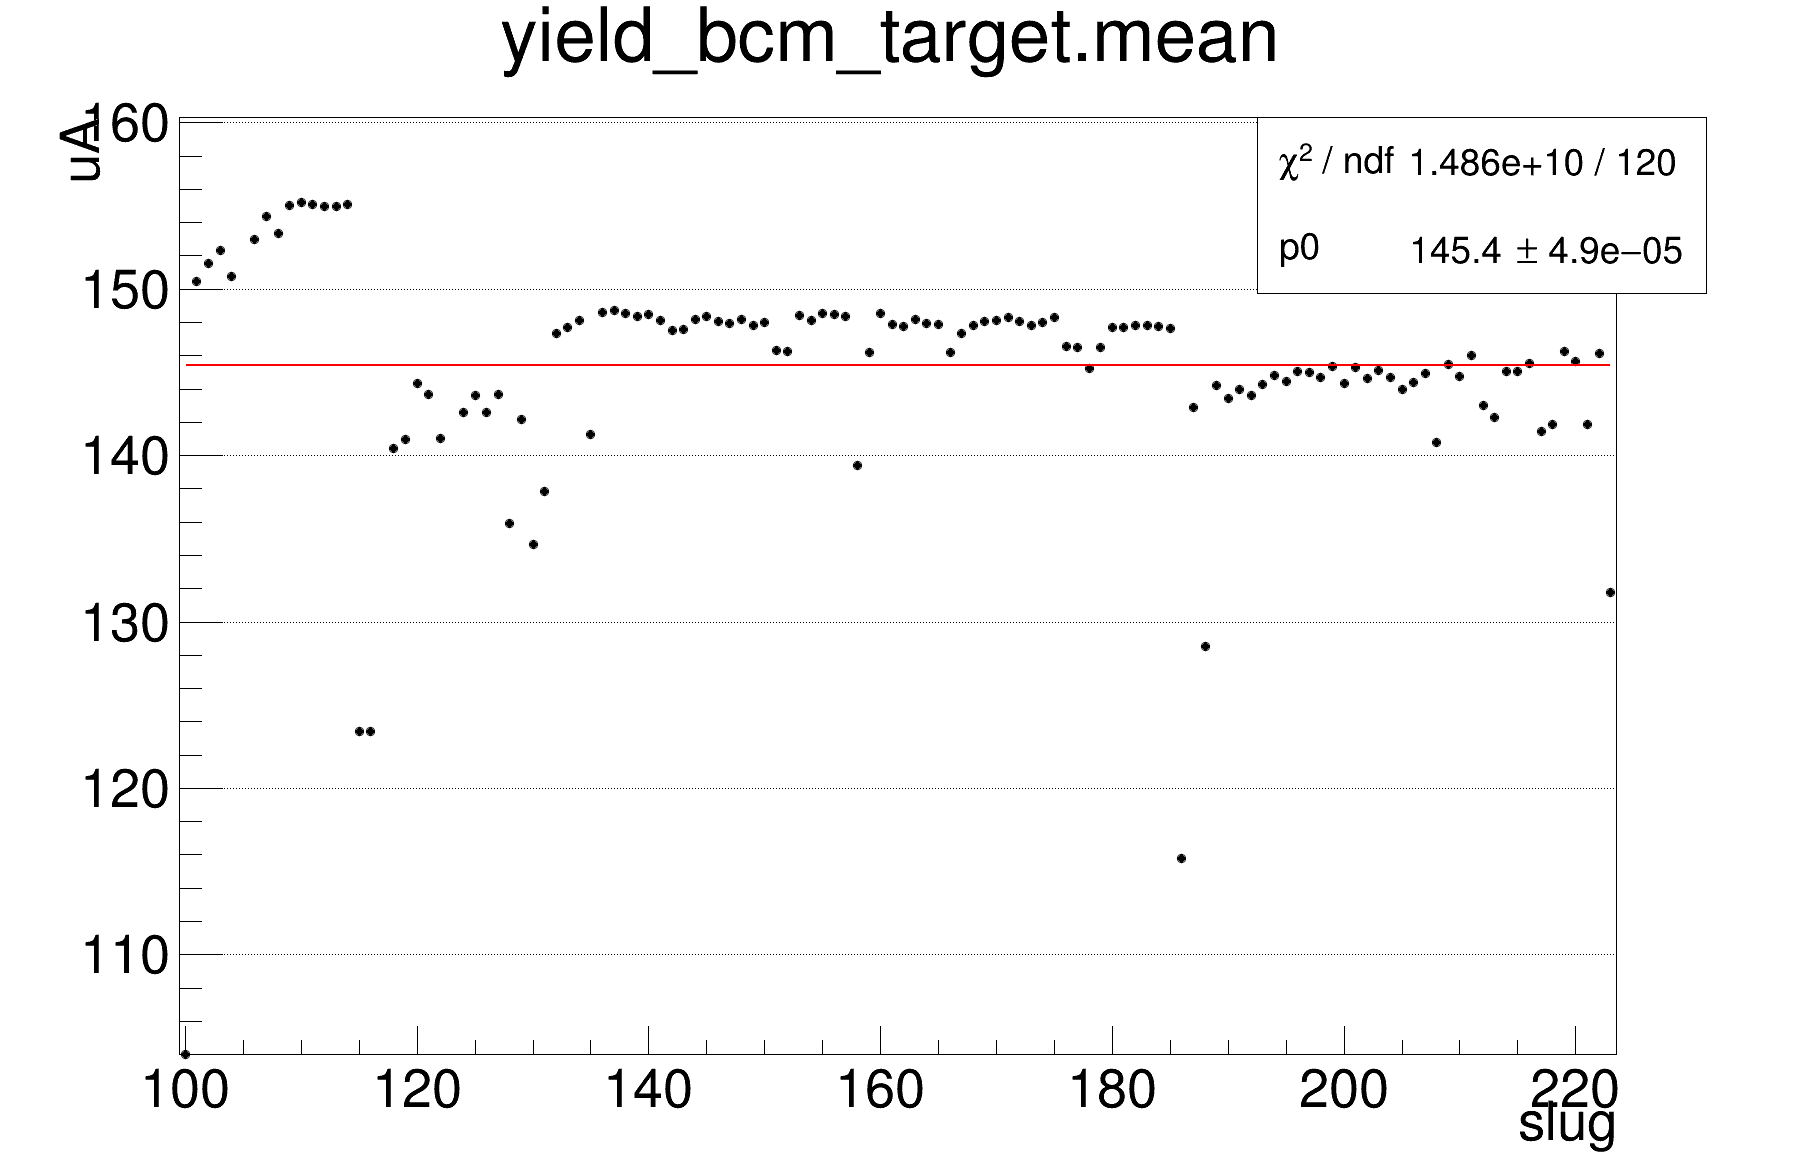
\includegraphics[width=0.32\linewidth]{crex_yield_bcm_target.mean}
    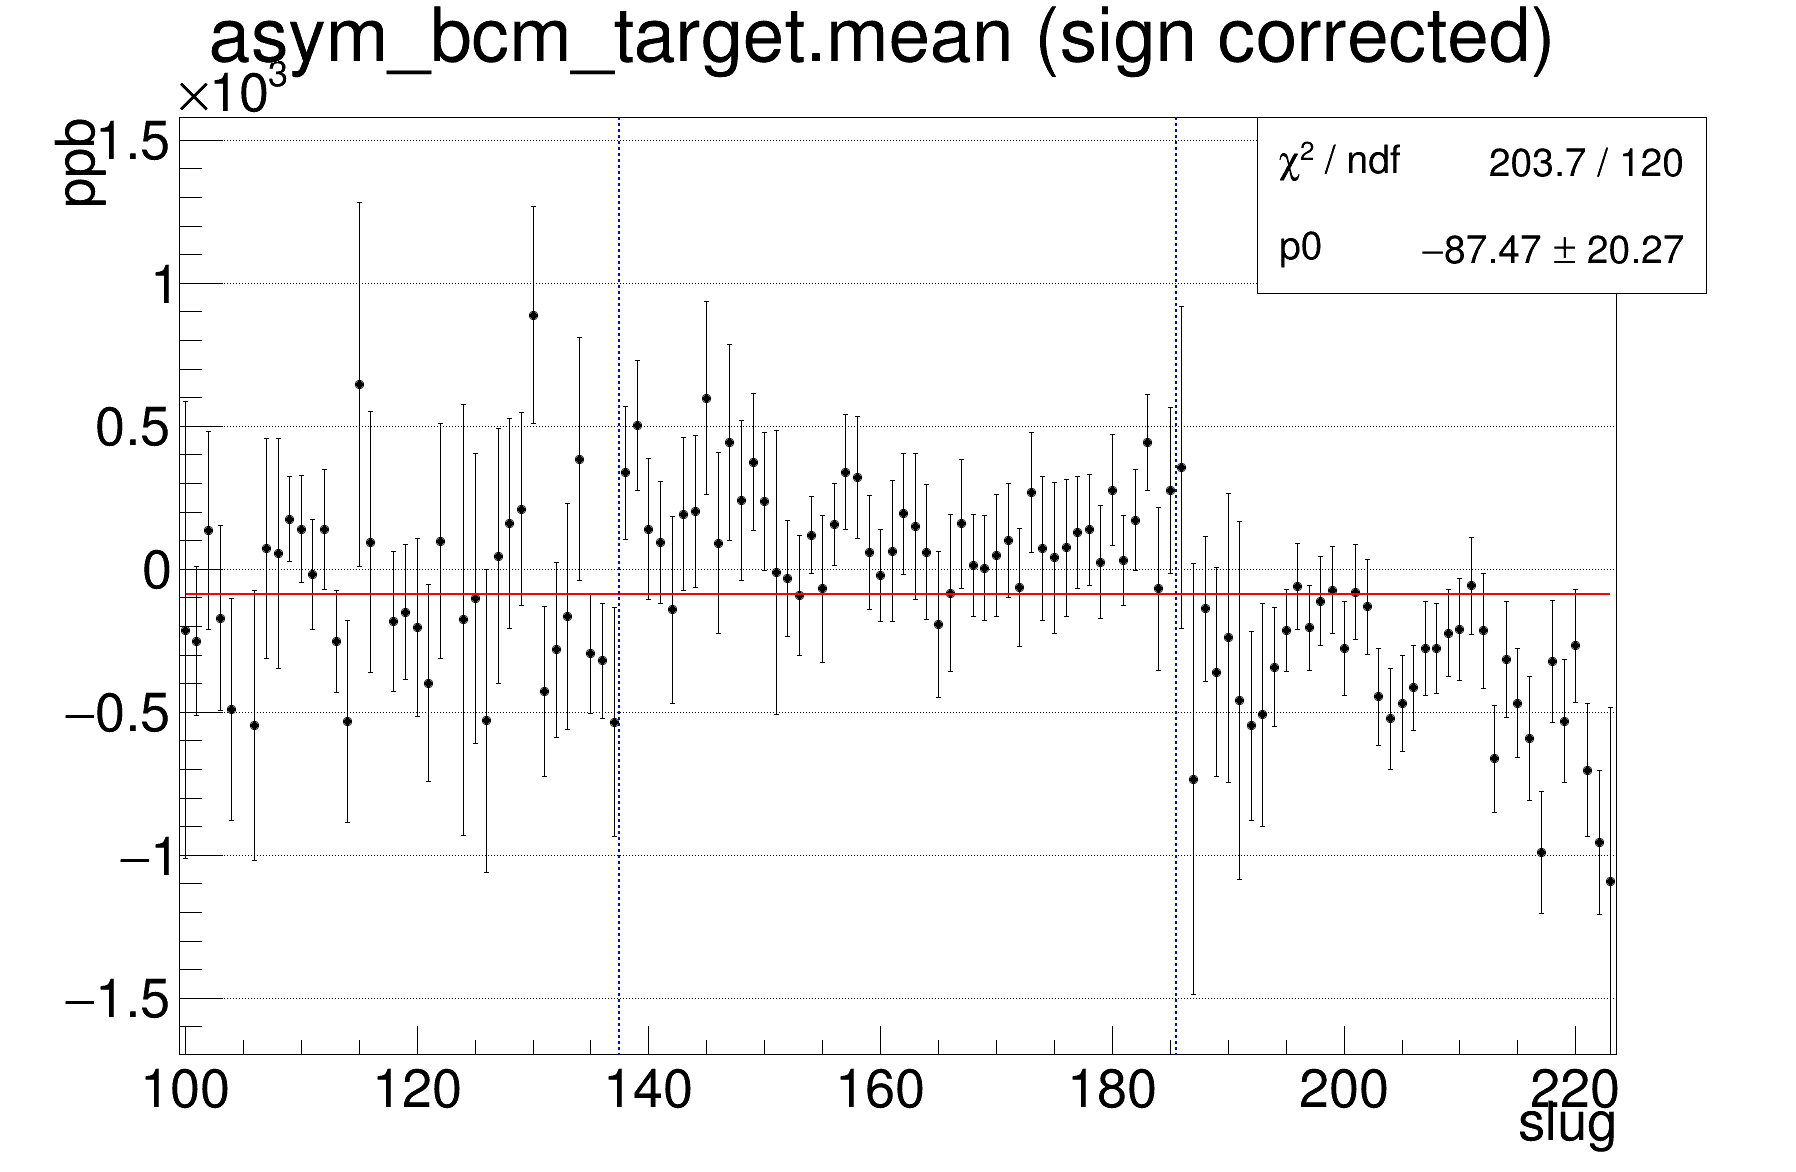
\includegraphics[width=0.32\linewidth]{crex_asym_bcm_target.mean}
    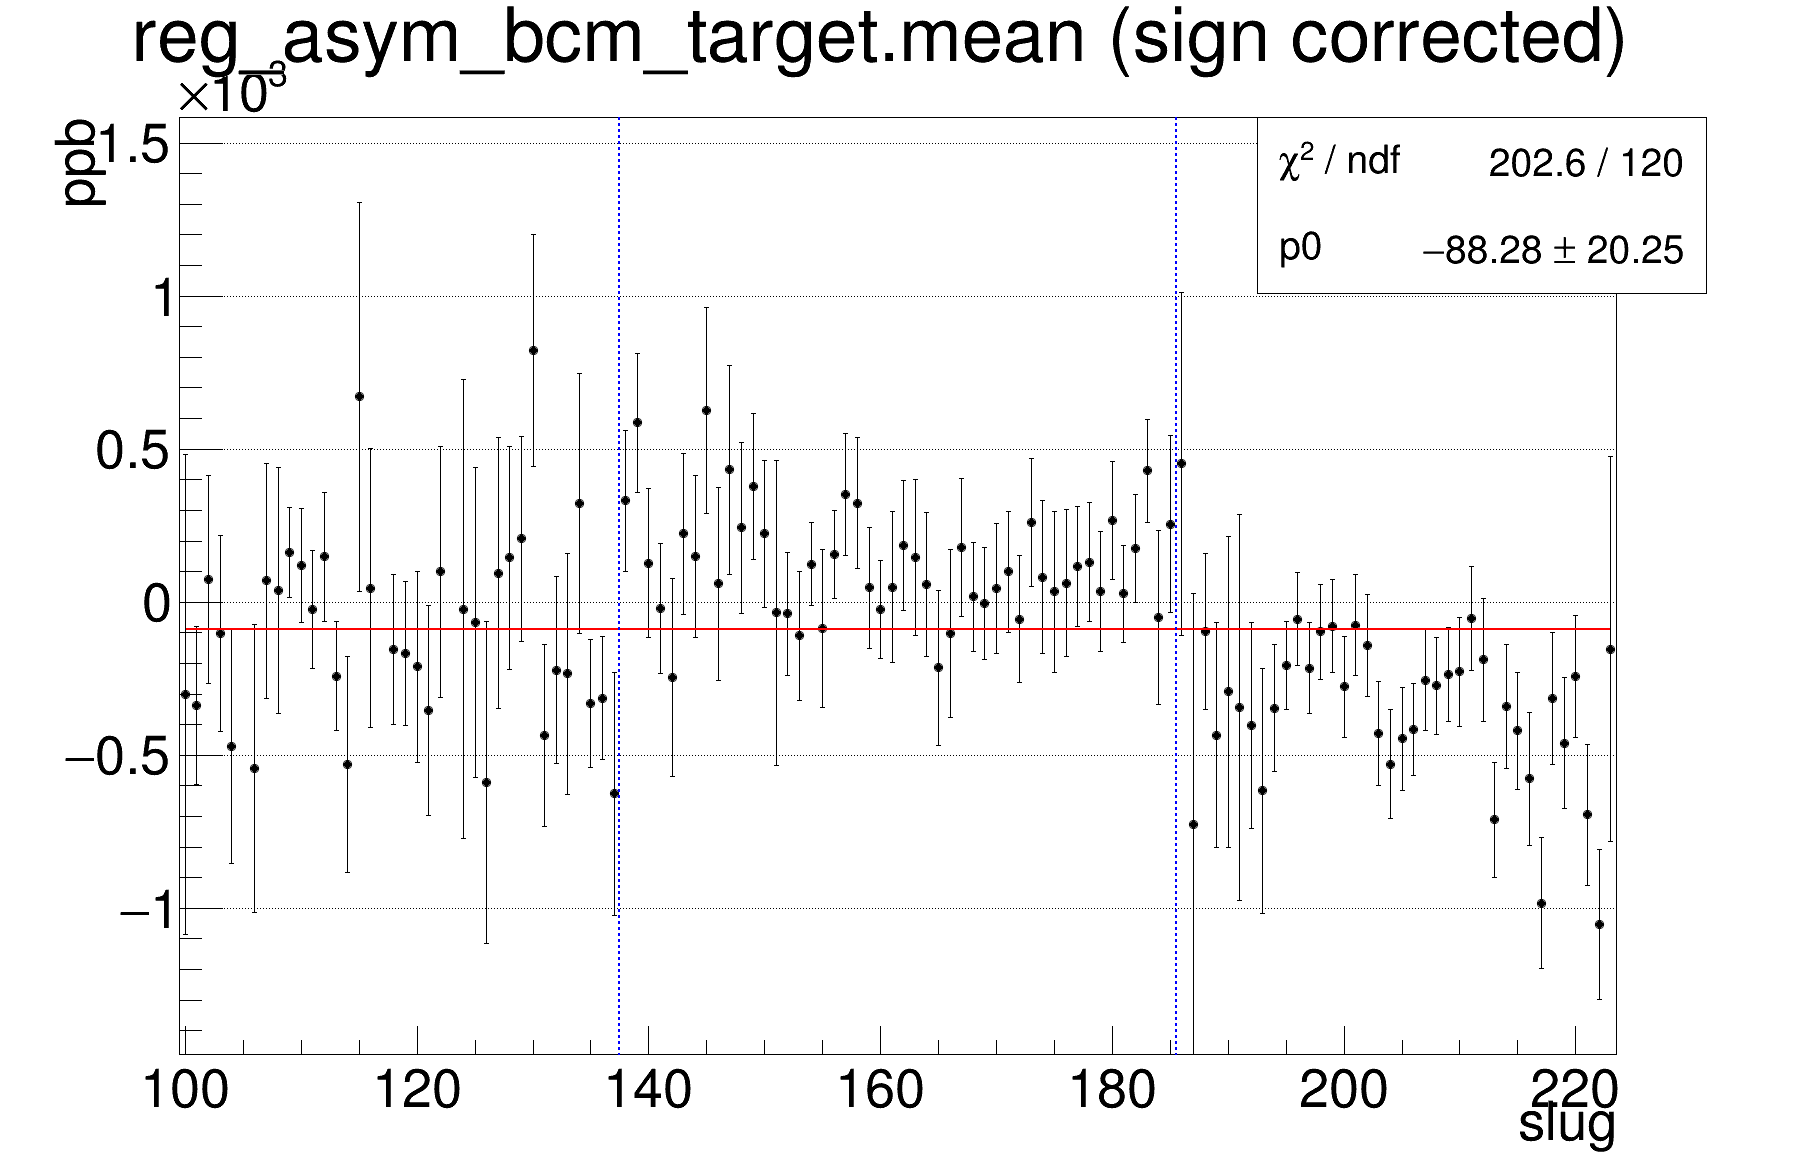
\includegraphics[width=0.32\linewidth]{crex_reg_asym_bcm_target.mean}
    \caption[Asymmetry slug-wise plot]
    {Slug-wise mean values of the beam current, asymmetry and regressed 
    asymmetry in CREX. The blue dashed lines separate
    the data set into three periods with different Wien-flip states.
    Most of the time, CREX run at $\sim 150\ \mu$A, an overall $\sim 100~$~ppb charge 
    asymmetry is achieved.}
    \label{fig:crex_bcm_target}
\end{figure}

%%%%%%%%%%%%%%%%%%%%%%%%
\subsubsection{Beam Position, Angle and Energy}
% target position/angle oscillation: http://ace.phys.virginia.edu/HAPPEX/4520
We do not have a direct measurement of the beam position and angle at the target, these 
information can be inferred from various BPMs. Given the 
distance between the target and BPM4a as $D1 = 5.725$~m and the distance
between BPM4a and BPM4e as $D2 =4.083$~m, the beam position and angle at the target 
will be:
\begin{equation}
    \begin{aligned}
	T_{X,Y} &= \text{BPM4a}_{X,Y} + \frac{\text{BPM4e}_{X,Y} - \text{BPM4a}_{X,Y}}{D2} D1	\\
	\theta_{X,Y} &= \frac{\text{BPM4e}_{X,Y} - \text{BPM4a}_{X,Y}}{D2} \\
    \end{aligned}
    \label{eq:target_pos}
\end{equation}
Using Eq.~\ref{eq:target_pos}, the overall difference of the beam position/angle 
at the target is calculated to be:
\begin{equation*}
    \text{diff}_{X,Y} \sim 10\ \mathrm{nm}	\qquad \text{diff}_{\theta_{X,Y}} \sim \mathrm{nrad}	
\end{equation*}
Again, the second period has a more stable beam than the other two periods.

\begin{figure}[!h]
    \centering
    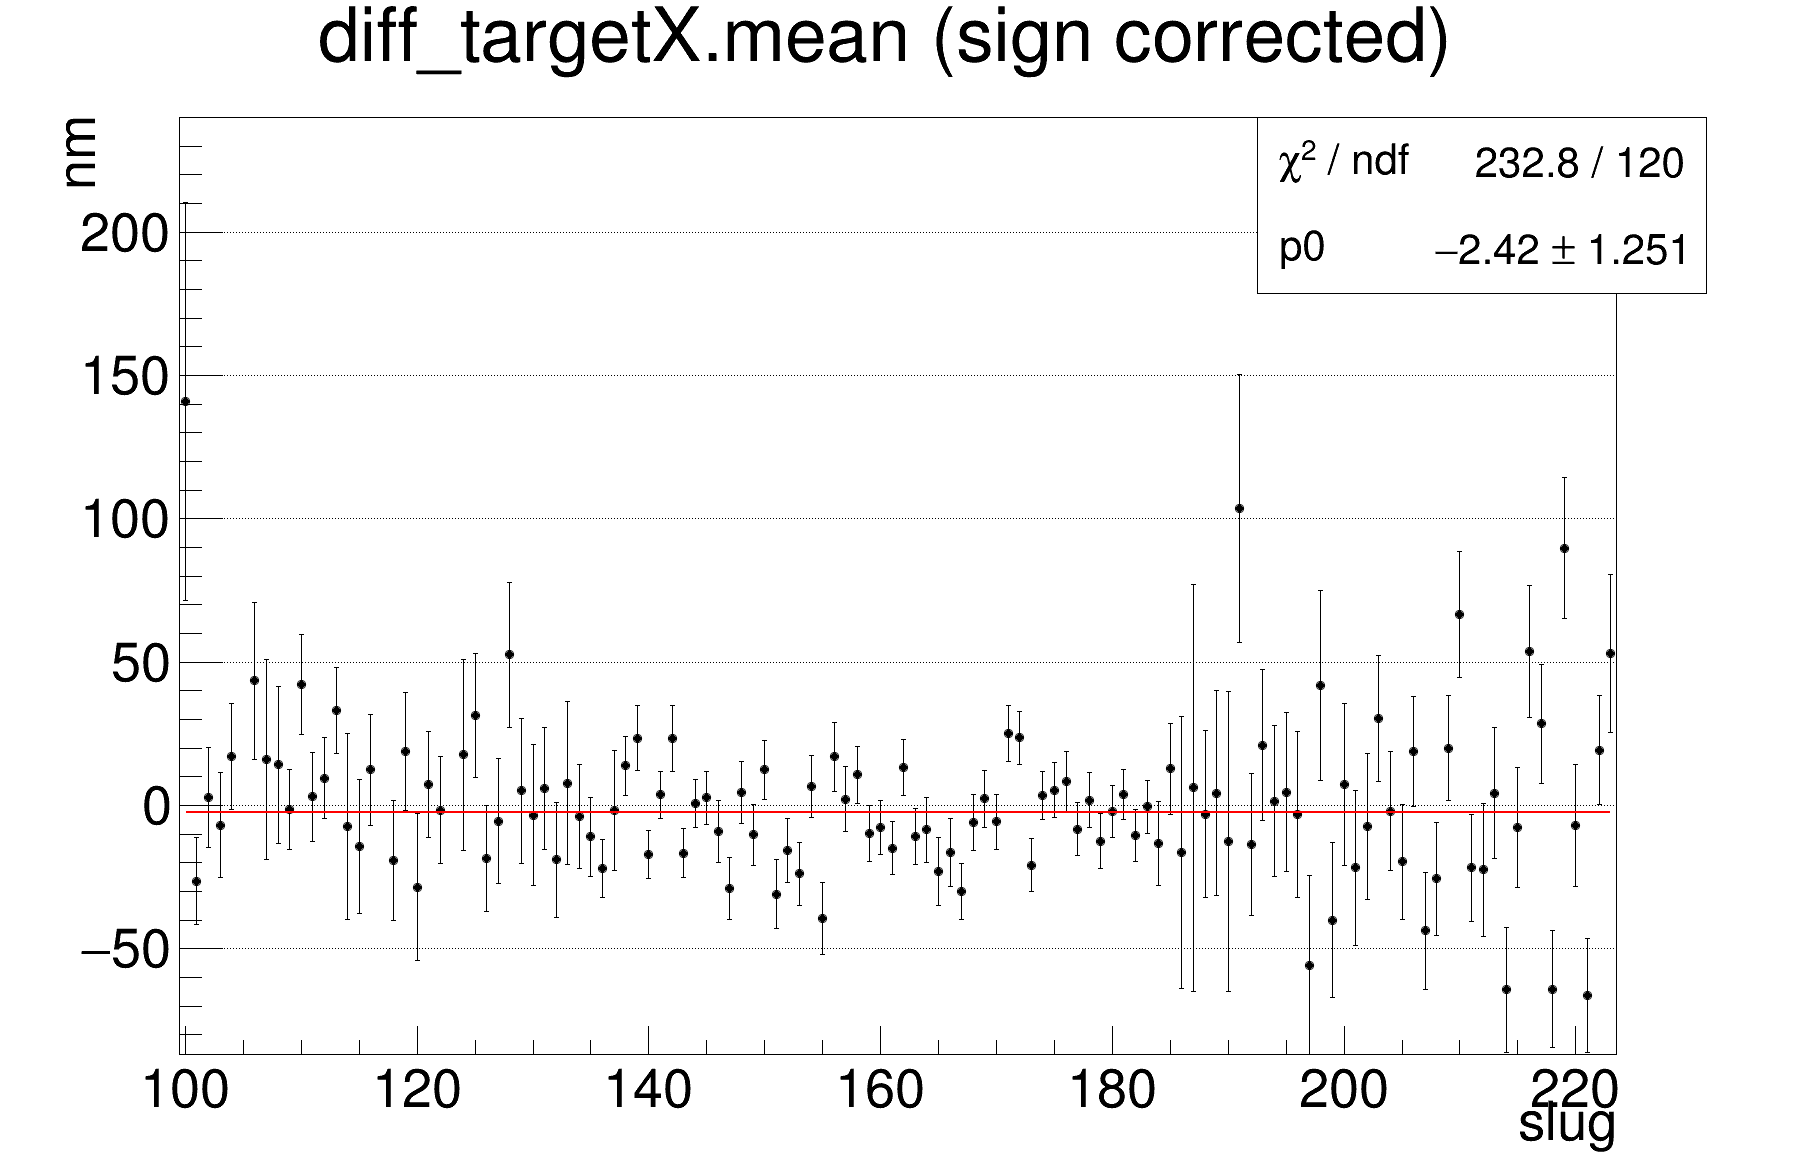
\includegraphics[width=0.49\linewidth]{crex_diff_targetX.mean}
    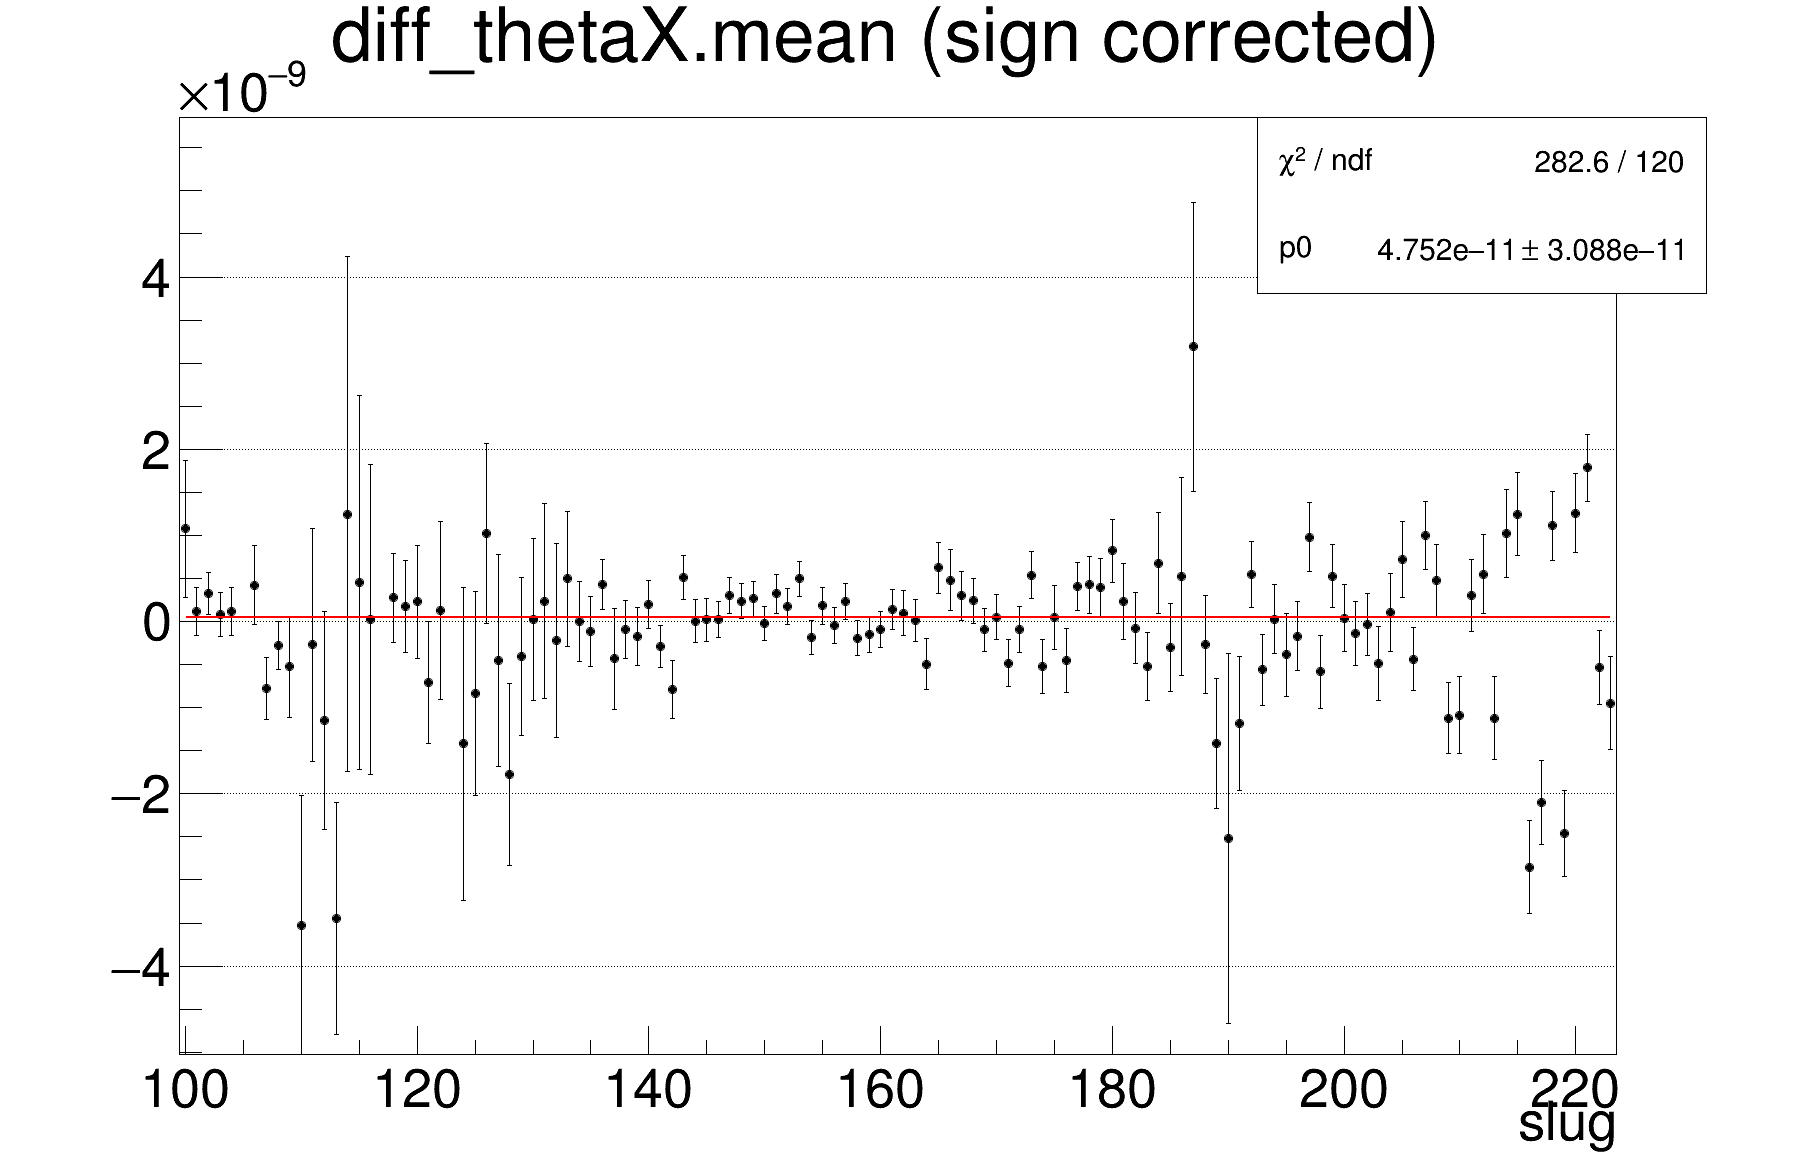
\includegraphics[width=0.49\linewidth]{crex_diff_thetaX.mean}
    \caption[Slug-wise plot of beam position and angle]
    {Slug-wise mean values of the beam position (left) and angle (right) 
    difference at the target. 
    Very precise control of the beam conditions is achieved.
    The Y dimension plots are similar and are not shown here.}
\end{figure}

The beam momentum/energy is measured by BPM12X, whose dispersion tells the deviation
(dp) from the standard momentum value (p0). The design value of the dispersion for CREX is
$D = 4.0$~m, and an actual measurement gives $\sim3.8$~m. I use 4.0~m here.
As can be seen in Fig.~\ref{fig:crex_diff_p}, CEBAF provides a beam with energy 
dispersion as small as $\sim10$~ppb.

\begin{equation}
    \frac{dp}{p} = \frac{\text{diff\_BPM12X}}{D}
\end{equation}

\begin{figure}[!h]
    \centering
    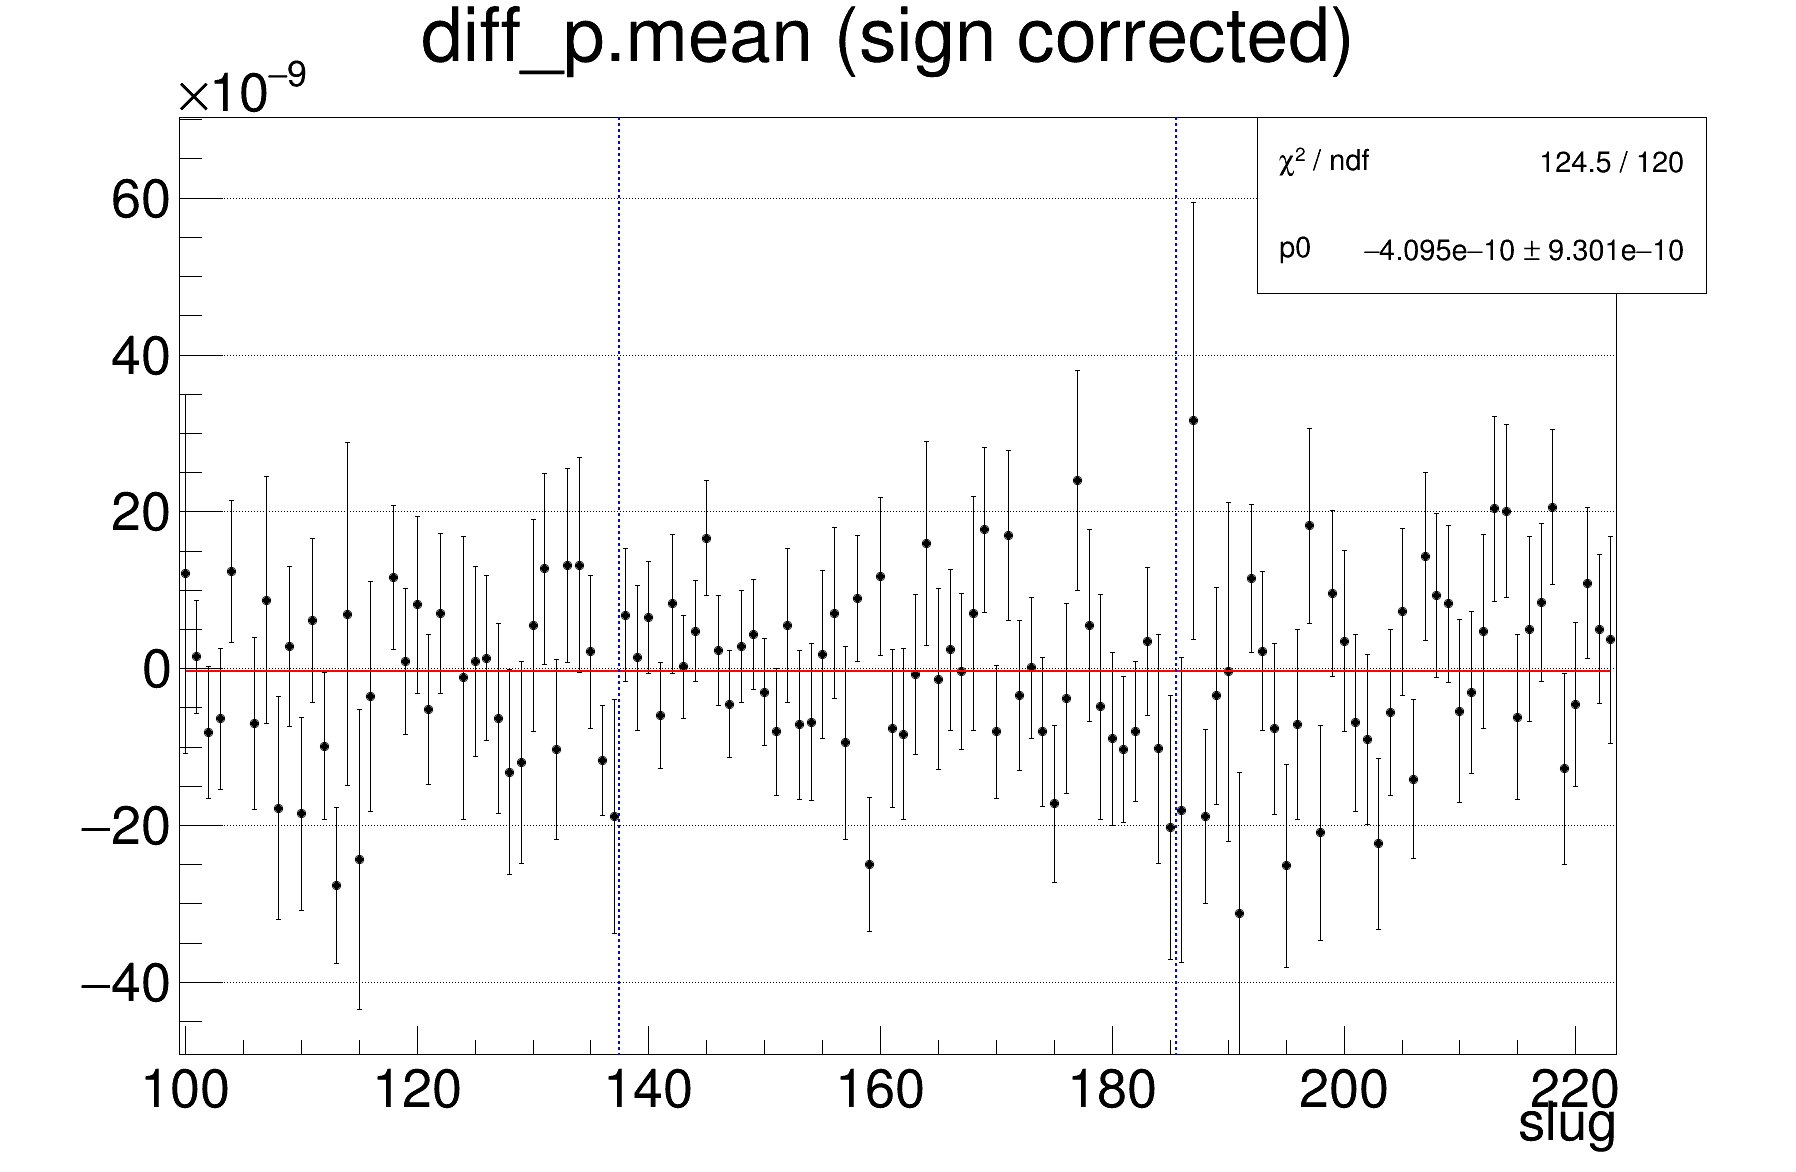
\includegraphics[width=0.6\linewidth]{crex_diff_p.mean}
    \caption{Slug-wise mean values of the beam energy dispersion. Overall, 
    an energy difference of $\sim 10$~ppb is achieved. }
    \label{fig:crex_diff_p}
\end{figure}

%%%%%%%%%%%%%%%%%%%%%%%%%%%%%%%%%%%%%%%%%%%%%%%%
\subsection{Raw Asymmetry}
% pedestal correction
The raw asymmetry is calculated as:
\begin{equation}
    \CA_{\text{raw}} \equiv 
    \begin{cases}
	\frac{d^+ - d^- - d^- + d^+}{d^+ + d^- + d^- + d^+}	& (+--+\ \text{pattern})    \\
	\frac{-d^- + d^+ + d^+ - d^-}{d^+ + d^- + d^- + d^+}	& (-++-\ \text{pattern})    \\
    \end{cases}
\end{equation}
where $d=\frac{D}{I}$ is the normalized detector integrating yield in one helicity
window, the upper-script indicates the helicity of the beam. The detector yield is
calibrated with their corresponding pedestals. 
% The raw asymmetry was blinded before the final result was freezed.
\begin{figure}[!h]
    \centering
    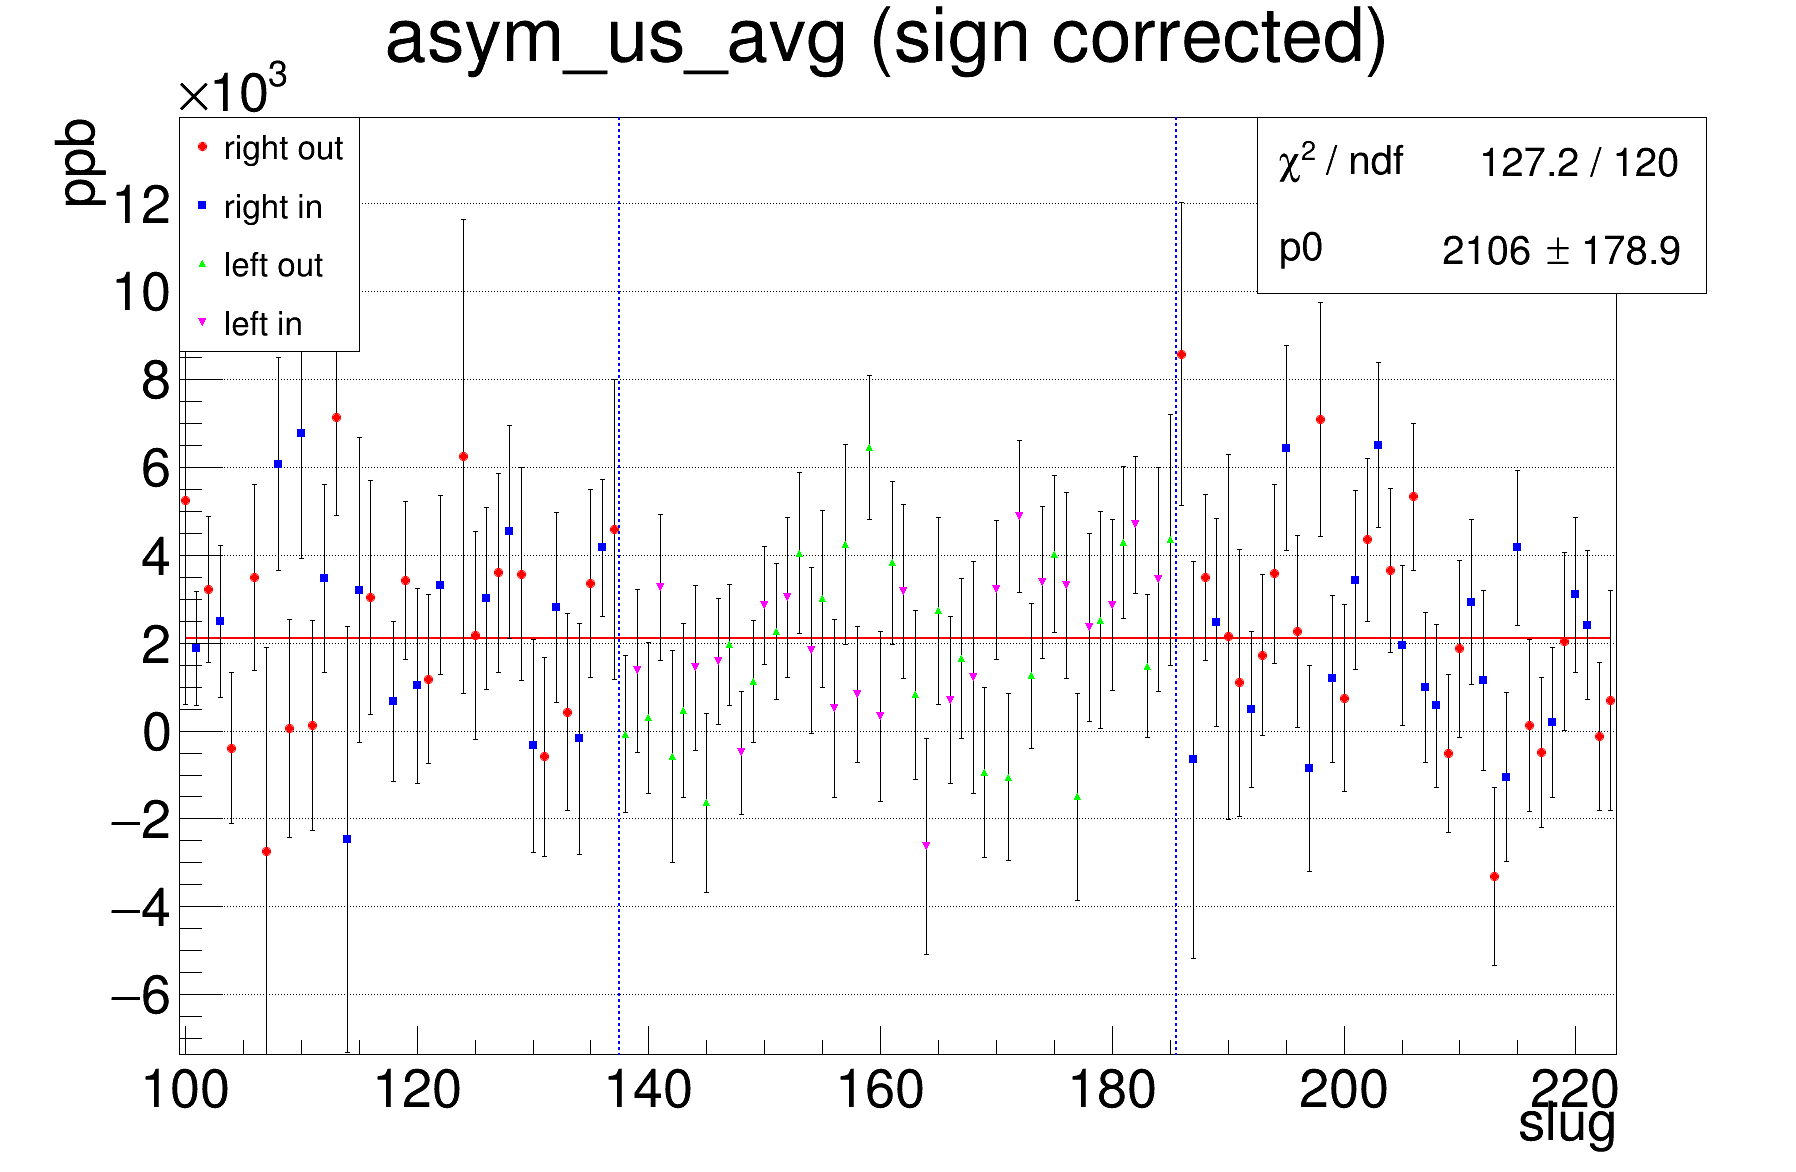
\includegraphics[width=0.49\linewidth]{crex_asym_us_avg}
    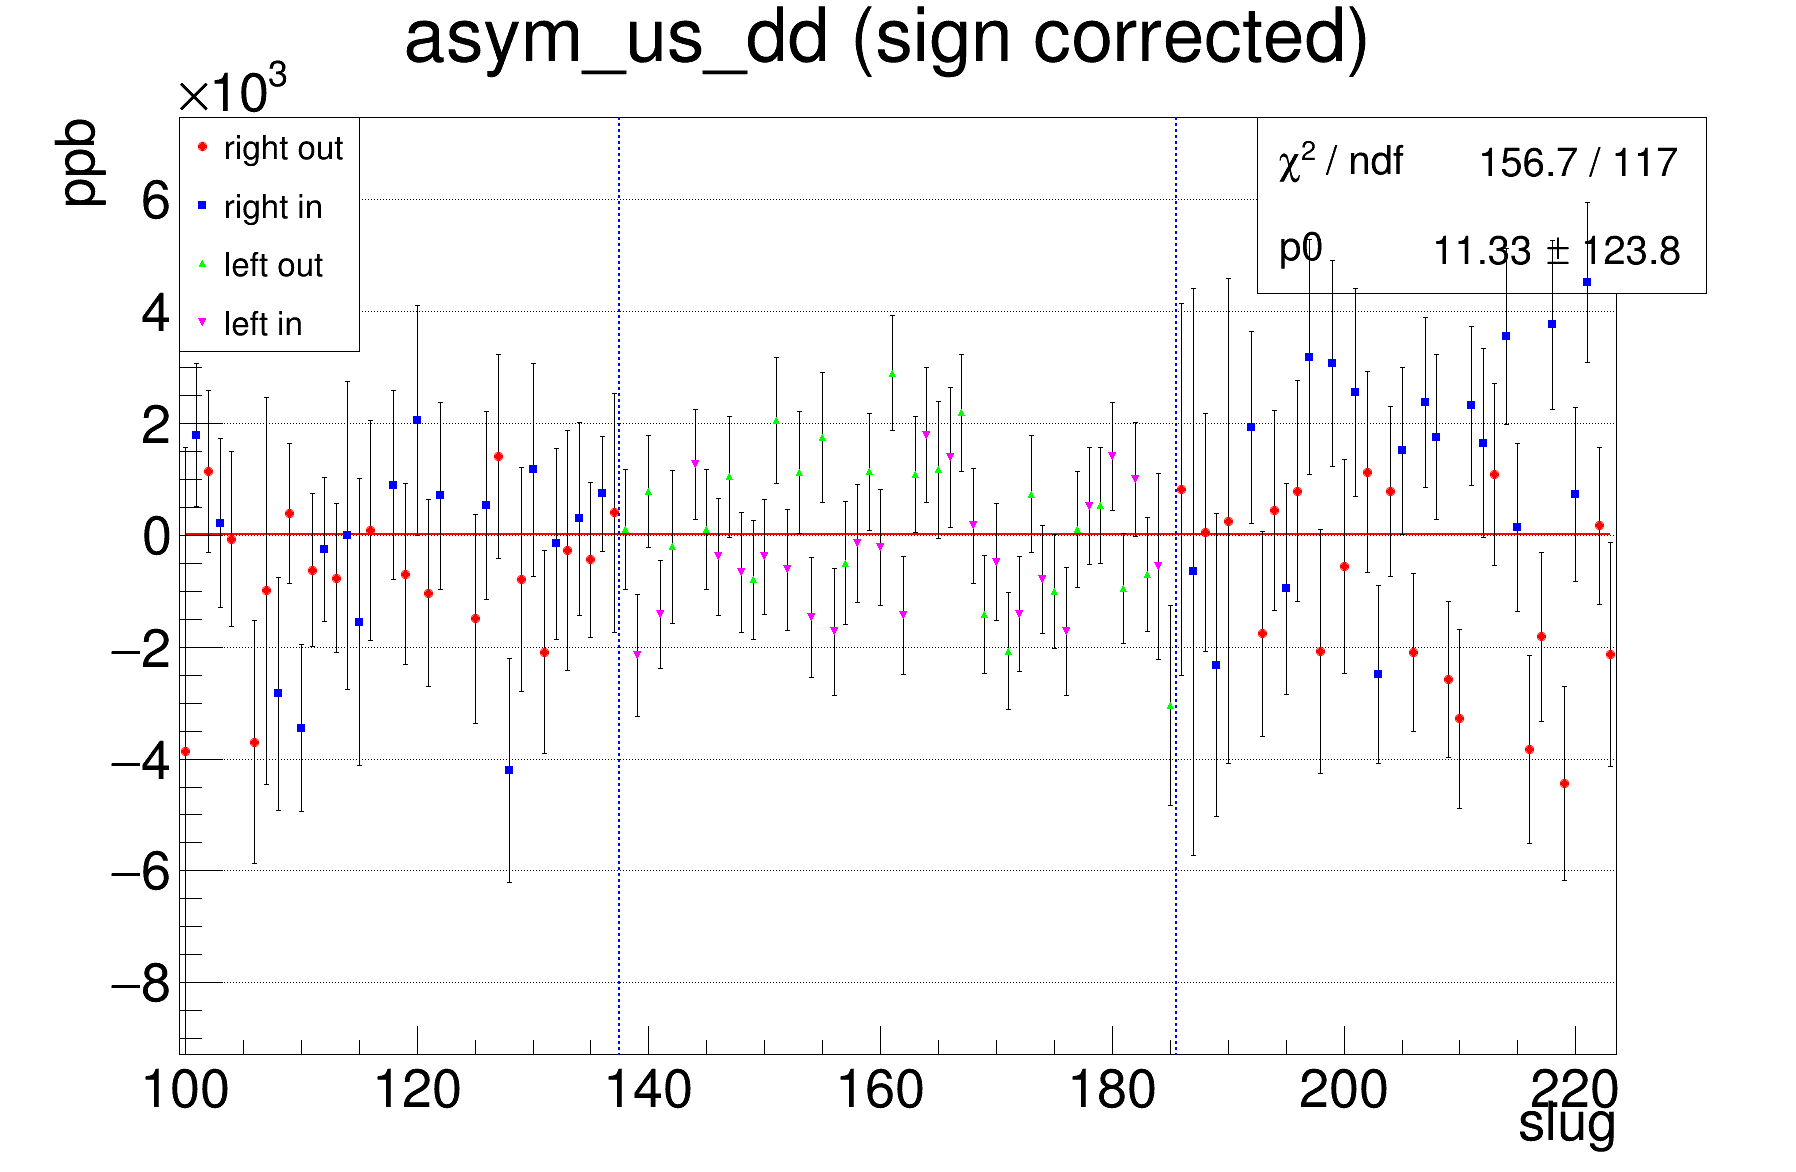
\includegraphics[width=0.49\linewidth]{crex_asym_us_dd}
    \caption{Slug-wise raw asymmetry average (left) and difference (right) for CREX. 
    The right plot has three less slugs because there are three single-arm slugs.}
\end{figure}

\begin{figure}[!h]
    \centering
    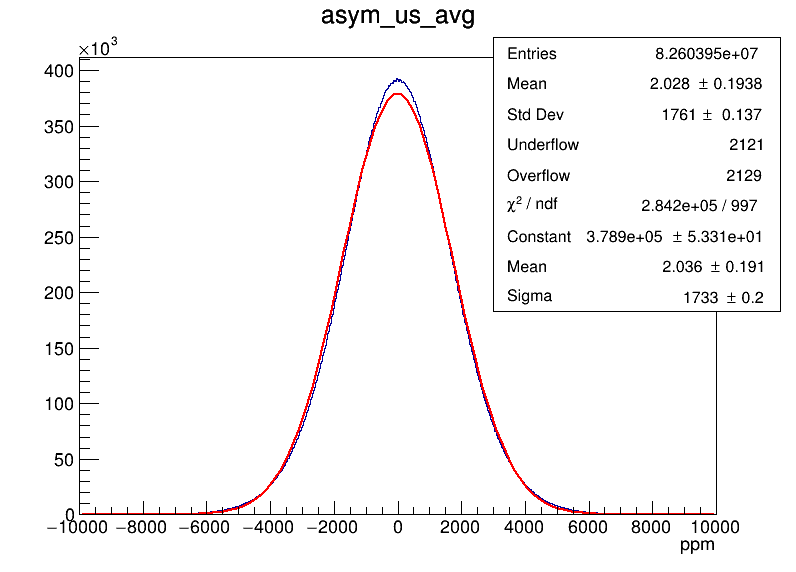
\includegraphics[width=0.49\linewidth]{crex_mulplot_asym_us_avg}
    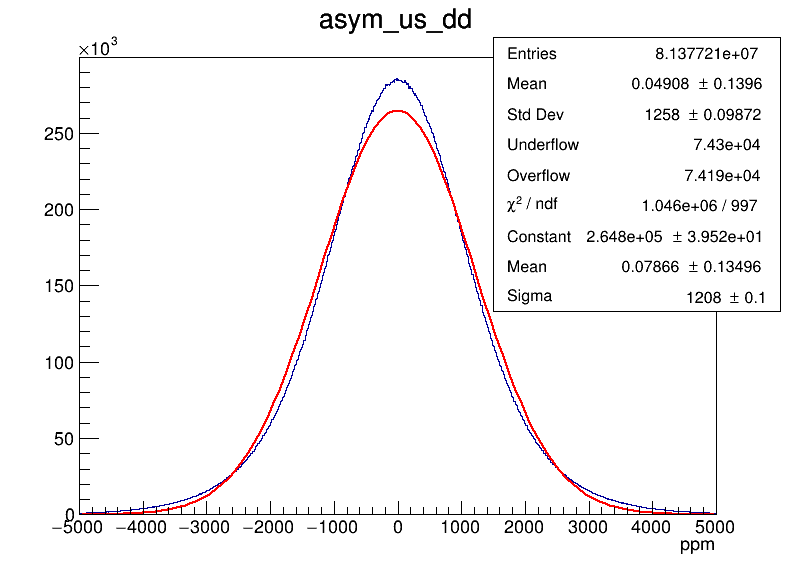
\includegraphics[width=0.49\linewidth]{crex_mulplot_asym_us_dd}
    \caption[Mulplots]
    {Mulplots of the CREX raw asymmetry average (left) and difference (right). 
    The blue line is the data and the red line is a Gaussian fit to the data. 
    The difference plot has less entries because single arm runs have no difference values.}
\end{figure}


%%%%%%%%%%%%%%%%%%%%%%%%%%%%%%%%%%%%%%%%%%%%%%%%%%%%%%%%%%%%%%%%%%%%%%%%
\section{Beam False Asymmetry Correction}
As shown in the previous few plots illustrating beam conditions, it is evident
that there are false asymmetries resulting from the beam. The primary contributor
is the helicity correlated beam asymmetry (HCBA).

As observed in Fig.~\ref{fig:correlation}, any beam jitter introduces
fluctuations in the detector yield, exhibiting approximately a linear correlation.
Therefore, to eliminate the false asymmetries caused by beam jitters, we just need to
know the correlation between the detector yield and each beam parameter, specifically
the detector slope. 

\begin{figure}[!h]
    \centering
    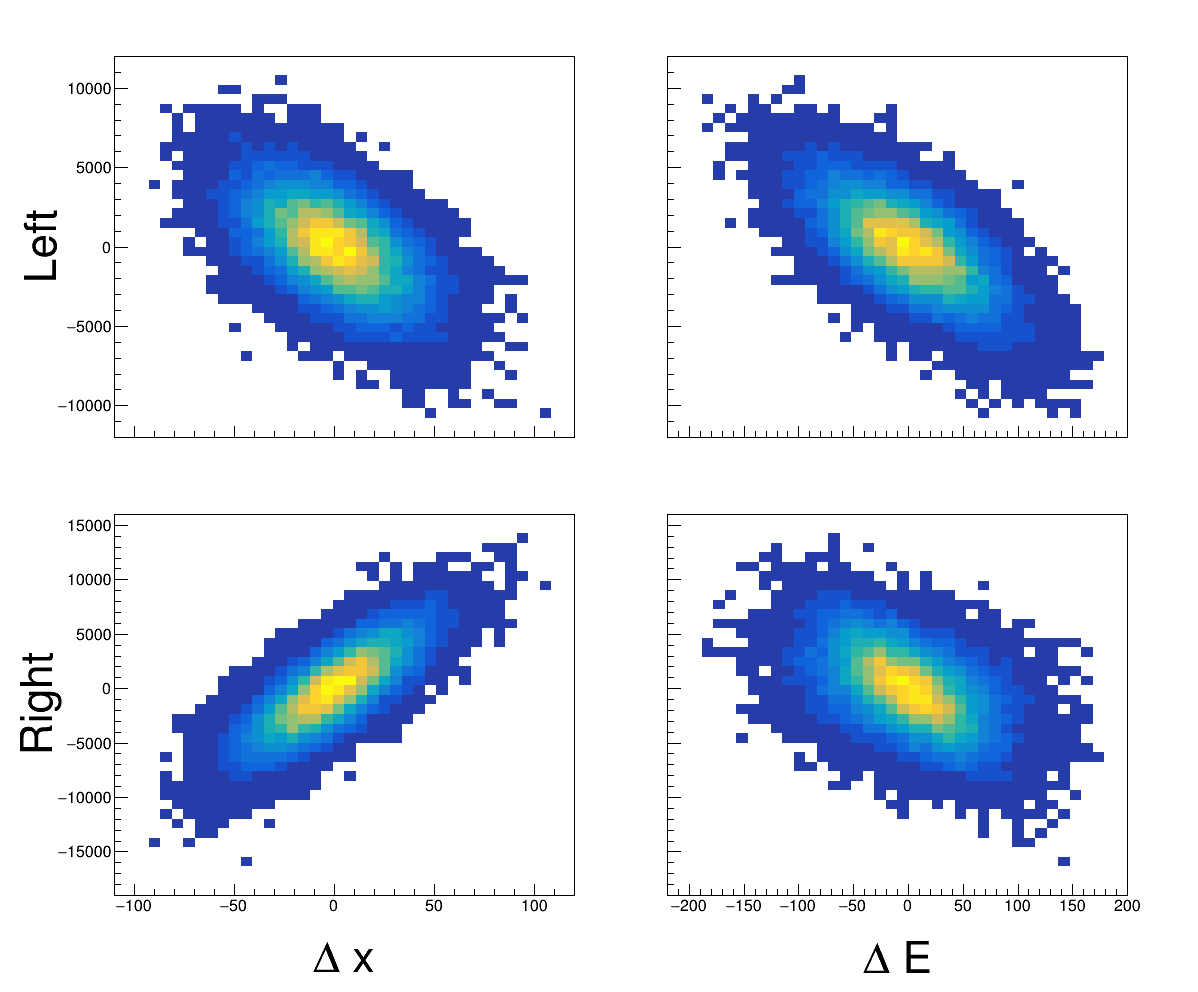
\includegraphics[width=0.6\linewidth]{run7679_correlation}
    \caption[Correlation plot in run 7679]
    {Correlation between the detector yield and the beam position/energy in run 7679.
    The left/right detector yields undergo opposite changes, when the beam position shifts,
    and they move in the same direction with respect to fluctuations in the beam energy.
    }
    \label{fig:correlation}
\end{figure}

There are 2 methods to calculate the slope values, regression and beam modulation,
we will delve into the details of these two methods in the following sections.

%%%%%%%%%%%%%%%%%%%%%%%%%%%%%%%%%%%%%%%%%%%%%%%%
\subsection{Regression}

The first method to calculate the slope is regression. Our data analysis 
provides a perfect scheme for the application of this statistical tool.

Bear in mind that regression alone does not establish relationships or rules.
Instead, it works based on the assumption that the relationship between variables 
is predictable (given by the user). Additionally, it assumes that the dependent 
variables follow a known distribution function $P(\epsilon)$, which is also provided by the user:
$$ Y = f(X) + \epsilon $$
With these prior knowledge, regression is capable of extracting the most likely 
coefficients in the predicted model.

\begin{comment}
For example, the famous least square fit is actually a linear regression 
$$ Y = c_0 + \sum c_i x_i + \epsilon $$
assuming Gaussian distribution of the dependent variable: $\epsilon \sim N(0, \sigma)$
Another frequently used scene is logistic regression for classification, which
is very similar to linear regression except f(X) will be converted into a
probability function, e.g. using the logistic function:
$$ h(z) = \frac{e^z}{1 + e^z} \quad z = f(X) $$

The assumption we made here is that the fluctuations in beam parameters in small, 
compared to their normal yield -- this can be verified by their yield plot. So
that we can use first order fit to model the detector's response to change in
beam parameters. Therefore the `true' asymmetry will be:
\begin{equation}
    \CA_{cor} = \CA_{raw} - \sum_i \beta_i\Delta M_i
\end{equation}
where $\CA_{cor}$ is the corrected asymmetry, $\beta_i = \frac{\partial \CA_{raw}}{\Delta M_i}$ 
is the slope and $\Delta M$ is the difference of BPM yield between 
opposite helicities windows, i sums over all 5 chosen BPMs.
\end{comment}

%%%%%%%%%%%%%%%%%%%%%%%%
\subsubsection{The Model}
Considering the scenario of only one monitor and one detector. 
Assuming that the reading noise of the detector
follows a Gaussian distribution and the monitor is precise (one can absorb the monitor
noise into the beam fluctuation):
\begin{equation}
    \begin{gathered}
	M = m	\\
	D = d + \epsilon(0, \sigma_0^D)    \\
    \end{gathered}
\end{equation}
here, the capital letters (D and M) represent the measured values while the 
small letters (m and d) denote the true values. $\sigma_0^D$ 
is the variance of the noise in the detector.

Then the difference between beams of opposite polarization will follow also
the Gaussian distribution with a larger variance:
\begin{equation}
    \begin{gathered}
	\Delta M = M^+ - M^- = m^+ - m^- = \Delta m   \\
	\Delta D = D^+ - D^- = (d^+ + \epsilon(0, \sigma_0^D)) - (d^- + \epsilon(0, \sigma_0^D))
	    = \Delta d_0 + \epsilon(0, \sqrt{2}\sigma_0^D)
	    = \Delta d + \epsilon(0, \sigma_1^D) \\
    \end{gathered}
\end{equation}
Again, $\Delta m$ and $\Delta d$ are the real differences,
whereas $\Delta M$ and $\Delta D$ are the measured values.

The probability for measuring $\Delta D$ will be:
\begin{equation}
    \begin{gathered}
	P(\Delta D) = \frac{1}{\sigma_1^D\sqrt{2\pi}} e^{-\frac{1}{2}\left( \frac{\Delta D - \Delta d}{\sigma_1^D}\right)^2}    \\
    \end{gathered}
\end{equation}

We will have a collection of independent data points: $(\Delta M, \Delta D)_i$.
Our objective is to determine the relationship between $\Delta d$ and $\Delta m$: 
$\beta \equiv \frac{\partial d}{\partial m}$. Since $\Delta m$ is significantly
smaller compared to its normal yield, a first-order correlation is considered
precise enough for our analysis.

This is exactly a linear regression problem.
\begin{equation}
    \begin{gathered}
	\Delta d = 0 + \beta \Delta m	\\
	\CA_{\text{cor}} = \CA_{\text{raw}} - \beta\Delta M	\\
    \end{gathered}
    \label{eq:first_order_correlation}
\end{equation}
where $\CA_{\text{cor}}$ is the corrected asymmetry.

For any real data point $(\Delta m, \Delta d)_i$, the possibility to measure
$(\Delta M, \Delta D)_i$ is:
\begin{equation}
    \begin{gathered}
	P_i(\Delta D|\Delta M) = \frac{1}{\sigma_1^D\sqrt{2\pi}} 
	    e^{-\frac{1}{2}\left( \frac{\Delta D - \beta\Delta M}{\sigma_1^D}\right)^2}
    \end{gathered}
\end{equation}

For the accumulated data of one minirun, the total probability will be:
\begin{equation}
    P = \prod_i^n P_i(\Delta D|\Delta M) = \prod_i^n \frac{1}{\sigma_1^D\sqrt{2\pi}} 
	    e^{-\frac{1}{2}\left( \frac{\Delta D_i - \beta\Delta M_i}{\sigma_1^D}\right)^2}
\end{equation}

To maximize P, it is equivalently to minimize:
\begin{equation}
    \chi^2 = \sum_i (\Delta D - \beta\Delta M)_i^2
    \label{eq:regression_chi2}
\end{equation}
where i sums over all samples in one minirun.

Maximization of P with respect to $\beta$ means a zero derivative:
\begin{equation}
    \frac{\partial P}{\partial \beta} = P \times 
    \sum_i \frac{\Delta M_i}{\sigma_1^D} \left( \frac{\Delta D_i - \beta\Delta M_i}{\sigma_1^D}\right)
    = 0
\end{equation}
which gives $\beta$ as:
\begin{equation}
    \sum_i \Delta M_i (\Delta D_i - \beta\Delta M_i) = 0 
\end{equation}
$$ \Downarrow $$
\begin{equation}
    \beta = \frac{\sum \Delta D_i \Delta M_i}{\sum \Delta M^2_i}
\end{equation}

Extending the independent variable to be multi-dimensional, we have:
\begin{equation}
    \Delta D = \begin{pmatrix} \beta_1 & \beta_2 & \cdots & \beta_m \end{pmatrix} 
	\begin{pmatrix}
	    \Delta M^1	\\
	    \Delta M^2	\\
	    \vdots 	\\
	    \Delta M^m	\\
	\end{pmatrix}
	+ \epsilon(0, \sigma^D)
\end{equation}
where m is the number of BPMs used for the asymmetry analysis.
\begin{equation}
    \frac{\partial P}{\partial \beta_\nu} \propto \sum_i \Delta M_i^\nu (\Delta D_i - \sum_\mu \beta_\mu M_i^\mu) = 0
    \label{eq:mul_dim_derivative}
\end{equation}
Arrange Eq.~\ref{eq:mul_dim_derivative} in a matrix:
\begin{equation}
    \small
    \begin{pmatrix}
	\sum_i \Delta D_i \Delta M_i^1 \\
	\sum_i \Delta D_i \Delta M_i^2 \\
	\vdots	\\
	\sum_i \Delta D_i \Delta M_i^m \\
    \end{pmatrix}
    = 
    \begin{pmatrix}
	\sum_i \Delta M_i^1 \Delta M_i^1    & \sum_i \Delta M_i^1 \Delta M_i^2	&
	\cdots	& \sum_i \Delta M_i^1 \Delta M_i^m  \\
	\sum_i \Delta M_i^2 \Delta M_i^1    & \sum_i \Delta M_i^2 \Delta M_i^2	&
	\cdots	& \sum_i \Delta M_i^2 \Delta M_i^m  \\
	\vdots	& \vdots    & \ddots	& \vdots    \\
	\sum_i \Delta M_i^m \Delta M_i^1    & \sum_i \Delta M_i^m \Delta M_i^2	&
	\cdots	& \sum_i \Delta M_i^m \Delta M_i^m  \\
    \end{pmatrix}
    \begin{pmatrix}
	\beta_1 \\
	\beta_2 \\
	\vdots	\\
	\beta_m \\ 
    \end{pmatrix}
\end{equation}

Define the covariance of any two variables as:
\begin{equation}
    \text{cov}(x, y) = \sum_i x_i y_i
\end{equation}
and
\begin{equation}
    M_{m \times m} = 
    \begin{pmatrix}
	\text{cov}(\Delta M^1, \Delta M^1) & \text{cov}(\Delta M^1, \Delta M^2)   & \cdots & \text{cov}(\Delta M^1, \Delta M^m)  \\
	\text{cov}(\Delta M^2, \Delta M^1) & \text{cov}(\Delta M^2, \Delta M^2)   & \cdots & \text{cov}(\Delta M^2, \Delta M^2)  \\
	\vdots	& \vdots    & \ddots	& \vdots    \\
	\text{cov}(\Delta M^m, \Delta M^1) & \text{cov}(\Delta M^m, \Delta M^2)   & \cdots & \text{cov}(\Delta M^m, \Delta M^m)  \\
    \end{pmatrix}
    \label{eq:M_definition}
\end{equation}

The coefficient vector will be extracted as:
\begin{equation}
    \begin{pmatrix}
	\beta_1 \\
	\beta_2 \\
	\vdots	\\
	\beta_m \\ 
    \end{pmatrix}
    =
    M^{-1}
    \begin{pmatrix}
	\text{cov}(\Delta D, \Delta M^1)   \\
	\text{cov}(\Delta D, \Delta M^2)   \\
	\vdots	\\
	\text{cov}(\Delta D, \Delta M^m)   \\
    \end{pmatrix}
    \label{eq:slope}
\end{equation}

\begin{comment}
For multiple detectors, it is easy to get:
\begin{equation}
    \small
    \begin{aligned}
	\begin{pmatrix}
	    \beta_{11}	& \beta_{21}    & \cdots & \beta_{m1}	\\
	    \beta_{12}	& \beta_{22}    & \cdots & \beta_{m2}	\\
	    \vdots	& \vdots    & \ddots	& \vdots\\
	    \beta_{1n}	& \beta_{2n}    & \cdots & \beta_{mn}	\\
	\end{pmatrix}
	&= A^{-1}
	&\times
	\begin{pmatrix}
	    \text{cov}(\Delta D^1, \Delta M^1) & \text{cov}(\Delta D^2, \Delta M^1)   & \cdots	& \text{cov}(\Delta D^m, \Delta M^1)	\\
	    \text{cov}(\Delta D^1, \Delta M^2) & \text{cov}(\Delta D^2, \Delta M^2)   & \cdots	& \text{cov}(\Delta D^m, \Delta M^2)	\\
	    \vdots	& \vdots    & \ddots	& \vdots    \\
	    \text{cov}(\Delta D^1, \Delta M^n) & \text{cov}(\Delta D^2, \Delta M^n)   & \cdots	& \text{cov}(\Delta D^m, \Delta M^n)	\\
	\end{pmatrix}
    \end{aligned}
    \label{eq:slope}
\end{equation}
where $\beta_{ij}$ refers to detector i's response to change in monitor j.
\end{comment}

Both theoretically and practically, it is possible to cover the entire phase space
beam motion using only 5 BPMs.
The 5 BPMs we chose in CREX analysis were BPM1X, BPM4aY, BPM4eX, BPM4eY and BPM12X.

%%%%%%%%%%%%%%%%%%%%%%%%
\subsubsection{Slope Values}
Using Eq.~\ref{eq:slope}, the slope values with respect to to the selected BPMs can be calculated. 
Fig.~\ref{fig:slug_202_reg_asym_us_avg_diff_bpm12X} shows the asymmetry's response
to changes in the beam energy, providing justification for utilizing miniruns. 
As observed in the plot, miniruns within the same run may have different 
slope values, varying by a few percent. This variation is expected because the 
detector slope is not a constant, it depends on the detector yield. 
Remember Eq.~\ref{eq:first_order_correlation} is based on the assumption that 
the beam fluctuations are tiny. In cases where there are relatively large shifts in the 
beam, new slopes are needed. Therefore, a minirun-wise slope value is 
more stable than a run-wise one, enabling a more precise correction of false 
asymmetry. Furthermore, this implies that the regression correction is most effective
for handling small fluctuations around the mean value. It is imprecise to apply
the same correction for outliers. That's why we need to remove miniruns with beam condition outliers.
\begin{figure}[!h]
    \centering
    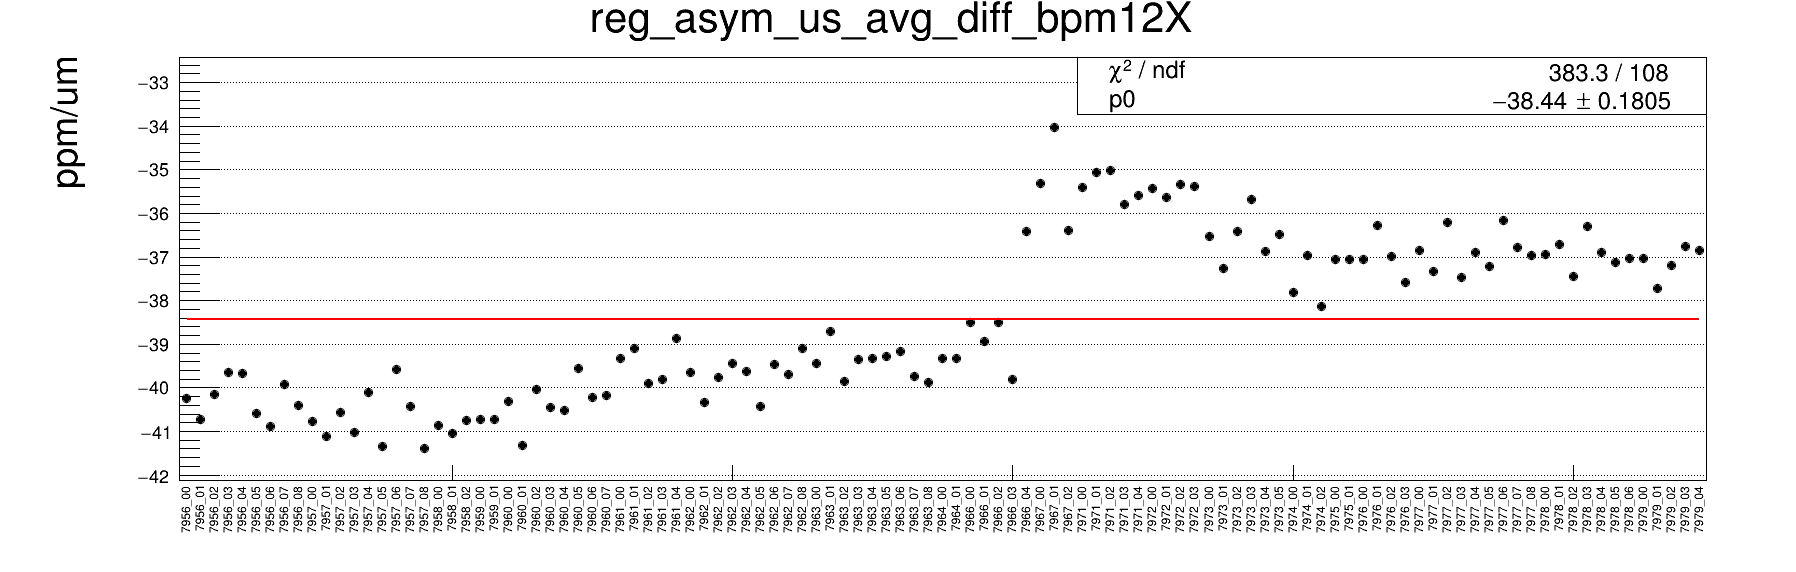
\includegraphics[width=\linewidth]{slug_202_reg_asym_us_avg_diff_bpm12X}
    \caption{Minirun-wise energy slope ($\partial$(asymmetry average)/$\partial$ (BPM12X)) 
    distribution in slug 202. The X-axis is the run number attached by a minirun number.}
    \label{fig:slug_202_reg_asym_us_avg_diff_bpm12X}
\end{figure}

Table~\ref{tab:crex_slope} summarizes the approximate slope values with respect to the 
five BPMs we chose. Overall, our detector exhibits sensitivity to fluctuations in the X direction, 
which is the dispersed direction, and the beam energy. On the other hand, the detector
is relatively insensitive to jitters in the Y direction.
\begin{table}[!h]
    \centering
    \begin{tabular}{c | c}
	\hline
	BPM & slope (ppm/$\mu$m)   \\
	\hline
	1X  & $\sim -40$    \\
	4aY & $\sim 15$    \\
	4eX & $\sim 40$	\\
	4eY & $\sim 0$	\\
	12X & $\sim -40$    \\
	\hline
    \end{tabular}
    \caption{Slope values of the asymmetry average with respcet to different BPMs.}
    \label{tab:crex_slope}
\end{table}

%%%%%%%%%%%%%%%%%%%%%%%%
\subsubsection{Corrections}
With the slope values, we can calculate the corresponding false asymmetry correction:
\begin{equation}
    \CA_{\text{false}} = \beta \times \text{(diff in BPM)}
\end{equation}
The primary correction comes from differences in the X direction and the beam energy.
A typical correction amounts to a few ppm, as shown in 
Fig.~\ref{fig:slug_202_reg_asym_us_avg_diff_bpm12X}.
Since the detector exhibits low sensitivity to fluctuations in the Y direction, 
the corresponding correction is relatively small, typically at the level of a few hundred ppb. 
Note that corrections from each beam parameter do not accumulate; instead, they 
cancel each other out, leading to a relatively small total correction, typically a few ppm.

\begin{figure}[H]
    \centering
    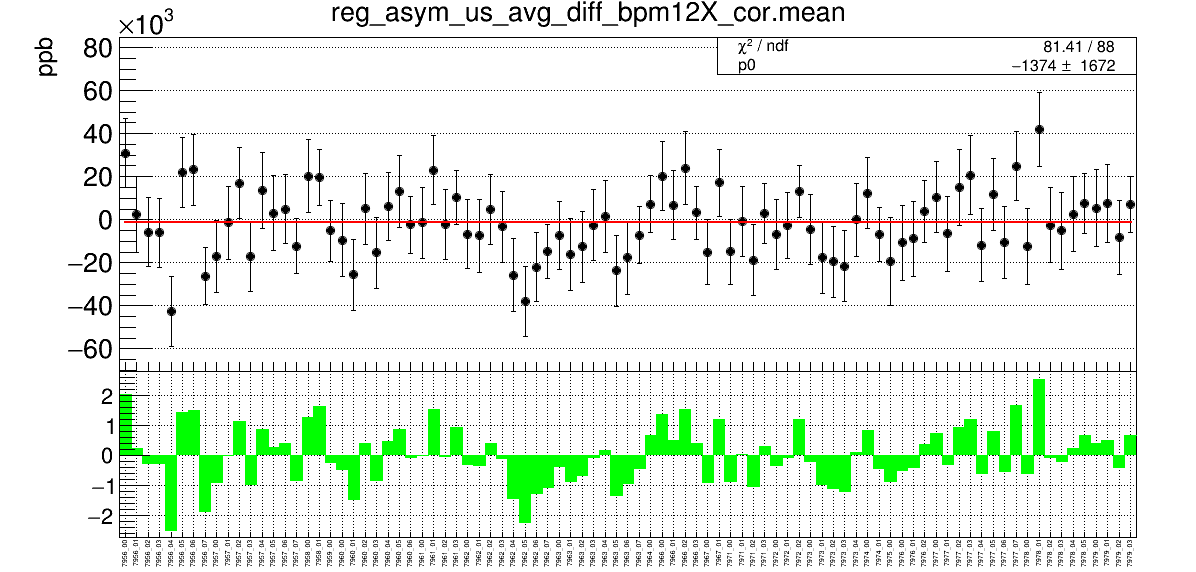
\includegraphics[width=\linewidth]{slug_202_reg_asym_us_avg_diff_bpm12X_cor.mean}
    \caption{False asymmetry correction caused by the energy difference (BPM12X) in
    slug 202.}
    \label{fig:slug_202_reg_asym_us_avg_diff_bpm12X_cor}
\end{figure}

\begin{table}[!h]
    \centering
    \begin{tabular}{c | c}
	\hline
	BPM  & correction   \\
	\hline
	1X  & a few tenths ppm \\
	4aY & a few hundreds ppb     \\
	4eX & a few tenths ppm \\
	4eY & a few hundreds ppb     \\
	12X  & a few tenths ppm \\
	\hline
    \end{tabular}
    \caption{Typical false asymmetry corrections from each BPM.}
\end{table}

%%%%%%%%%%%%%%%%%%%%%%%%
\subsubsection{Regression Result}
The asymmetry after the regression correction reads $2080 \pm 84.01$~ppb, as shown 
in the left plot of Fig.~\ref{fig:reg_asym_us_avg}. In Comparison, the raw asymmetry
without correction is measured as $2106 \pm 178.9$~ppb.

As expected, the mean value of the asymmetry does not change significantly after
regression correction. This outcome aligns with our assumption that the false 
asymmetry follows the Gaussian distribution. Therefore the regression correction
primarily removes noise without altering the mean value.
Moreover, the width of the asymmetry distribution considerably reduces by a 
factor of 2 after the regression correction, as shown in the right plot of Fig.~\ref{fig:reg_asym_us_avg}. This reduction in width indicates that the regression correction effectively diminishes the noise.

\begin{figure}[!h]
    \centering
    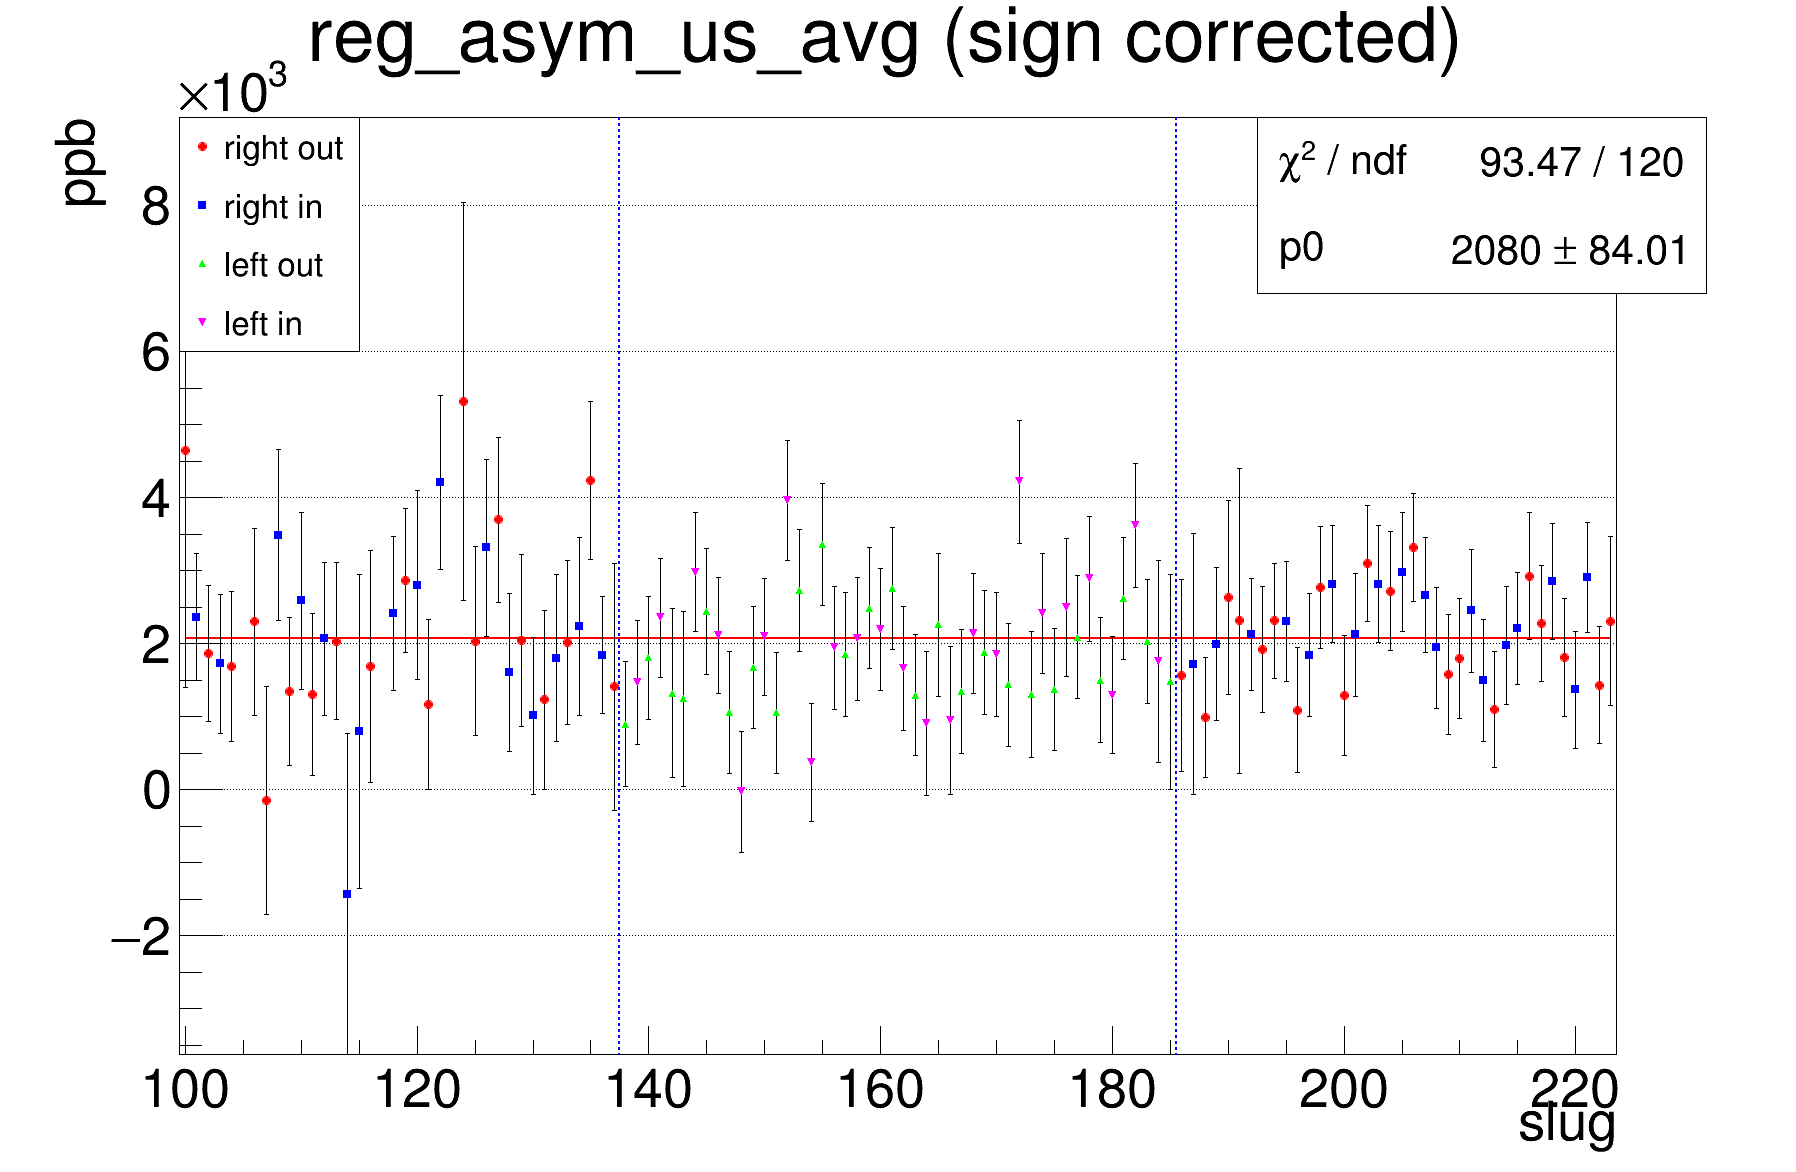
\includegraphics[width=0.52\linewidth]{crex_reg_asym_us_avg}
    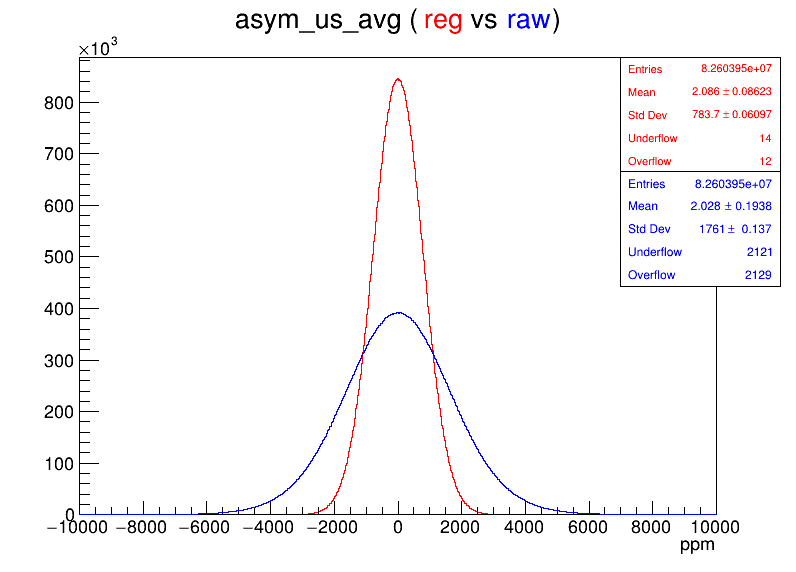
\includegraphics[width=0.47\linewidth]{crex_mulplot_asym_us_avg_cor}
    \caption[Regression correction asymmetry]
    {Left: slug-wise scatter plot of the asymmetry values after the regression correction.
    Right: Comparison of the experiment-wise distributions of the asymmetry values
    before and after the regression correction.}
    \label{fig:reg_asym_us_avg}
\end{figure}

%%%%%%%%%%%%%%%%%%%%%%%%
\subsubsection{Null Result}
A reliable method for verifying the correctness of our result is by examining the 
null asymmetry, which is calculated as the difference between the LHRS and RHRS 
asymmetries divided by 2. 
In an ideal case, the null asymmetry should be zero. Our measurement shows exactly
this expectation, the regression-corrected null asymmetry is about 85~ppb, which
is very close to zero.
\begin{figure}[!h]
    \centering
    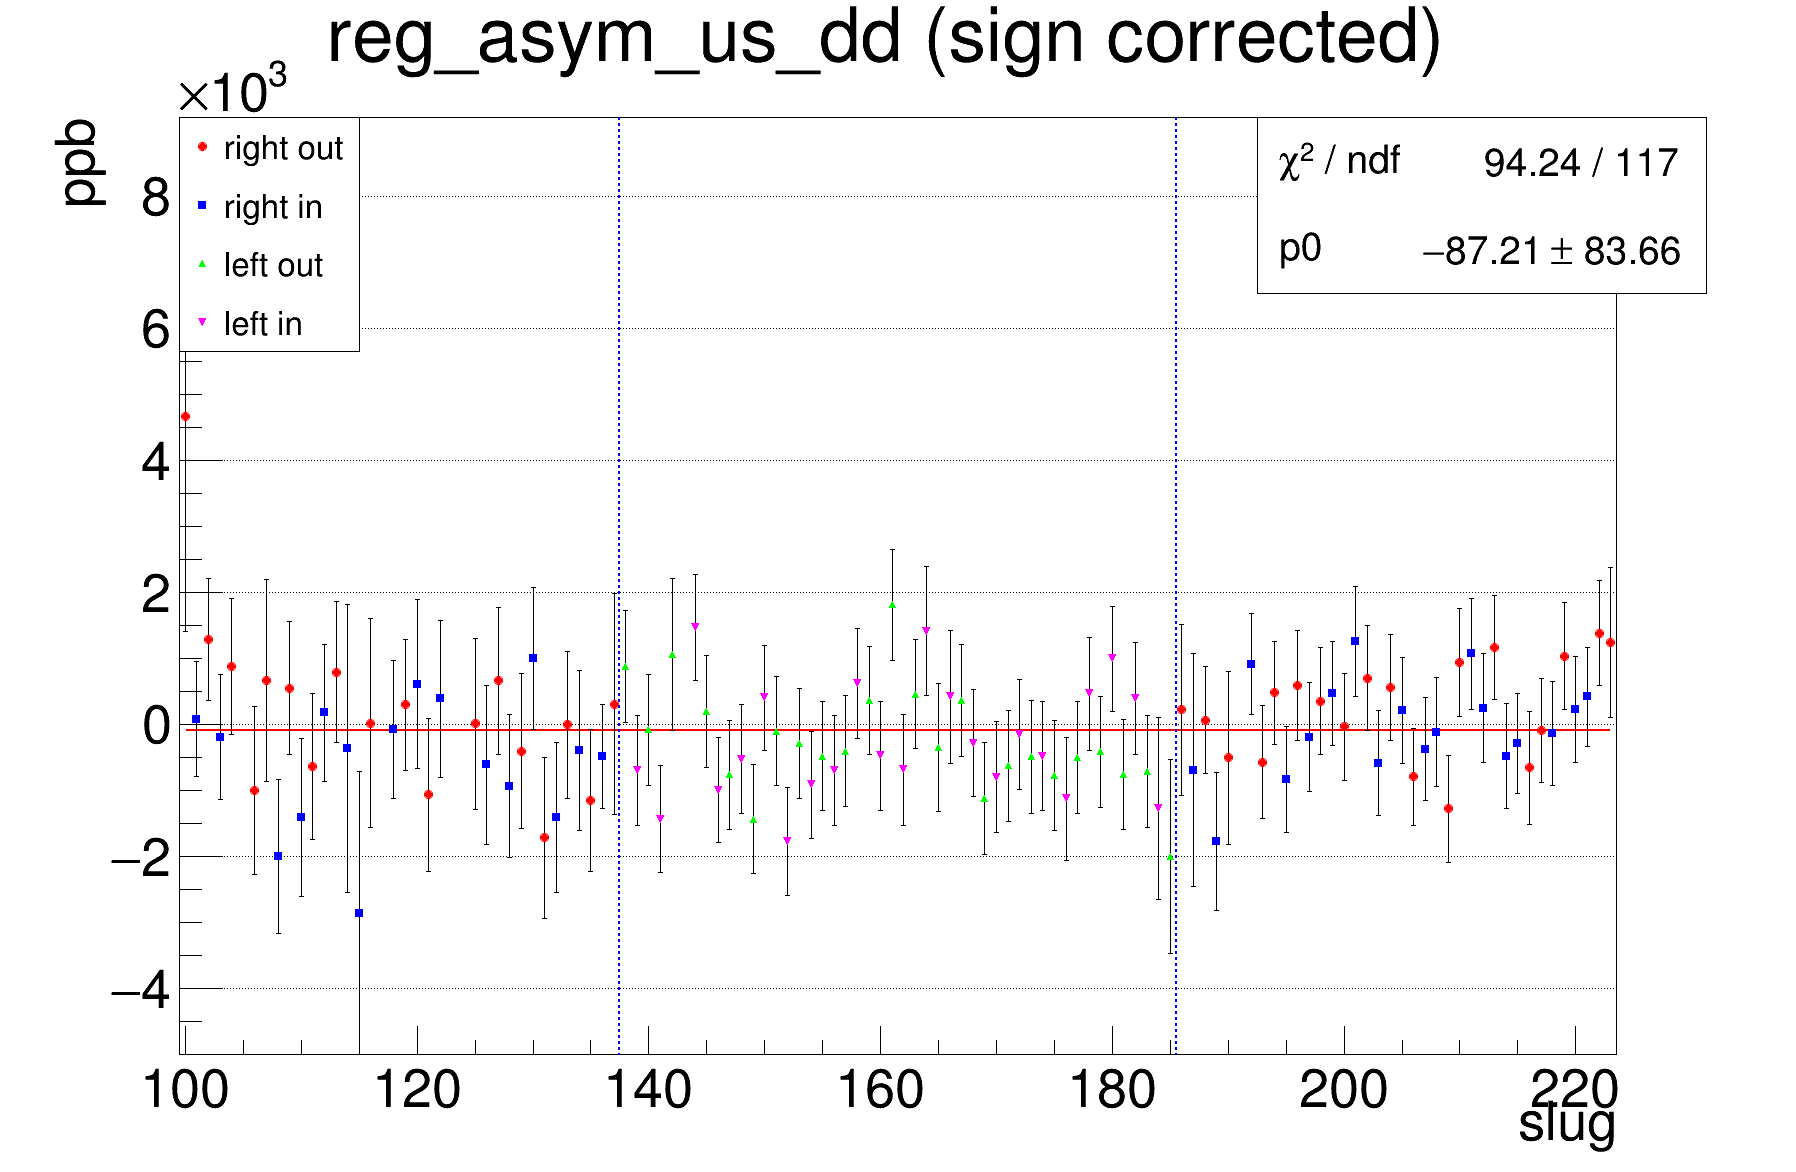
\includegraphics[width=0.52\linewidth]{crex_reg_asym_us_dd}
    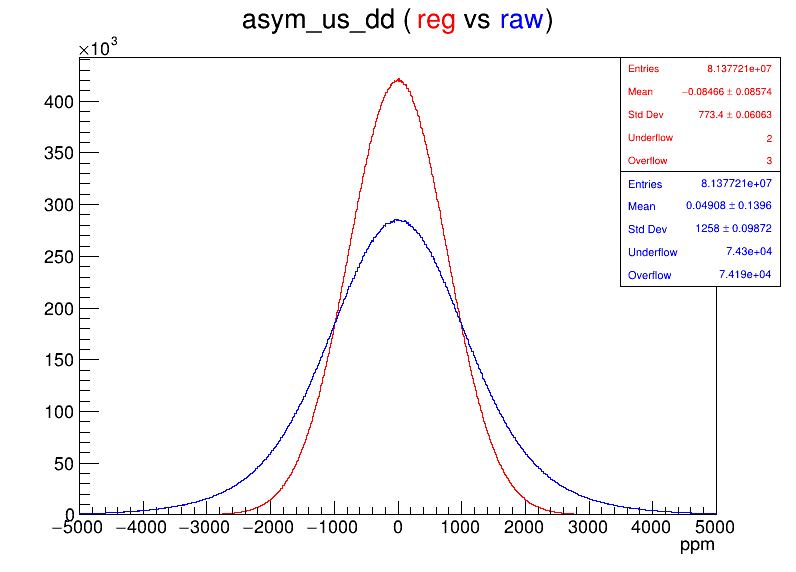
\includegraphics[width=0.47\linewidth]{crex_mulplot_asym_us_dd_cor}
    \caption{Slug-wise scatter plot (left) and experiment-wise histogram (right) of the
    regression-corrected null asymmetry.}
    \label{fig:reg_asym_us_dd}
\end{figure}

%%%%%%%%%%%%%%%%%%%%%%%%%%%%%%%%%%%%%%%%%%%%%%%%
\subsection{Beam Modulation (Dithering)}
Another approach to correcting the beam false asymmetry is through beam modulation. 
This method involves intentionally modulating the beam position, angle, or energy to directly measure the detector's response to the beam fluctuations. By observing the changes in the monitors and detectors during the modulation, we can determine the slope values.
The key point is to make sure that the amplitude of the modulation is larger 
than that of natural beam fluctuations. This is necessary to distinguish the true response of the detector from the inherent variability of the beam.

\begin{figure}
    \centering
    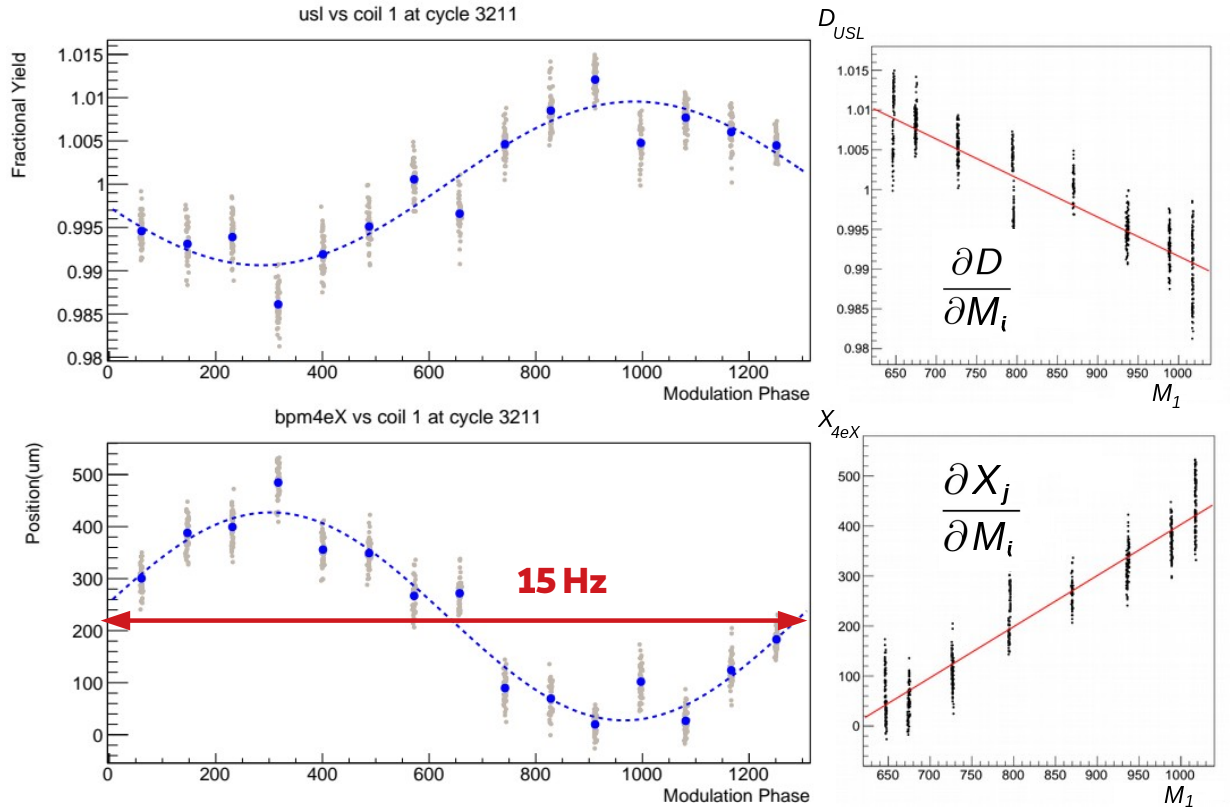
\includegraphics[width=0.7\linewidth]{modulation_cycle3211}
    \caption{An example of beam modulation.}
\end{figure}

To express the idea mathematically, let D (M) be the Detector (Monitor) yield and C be
the modulation coil input, we have:
\begin{equation}
    \frac{\partial D}{\partial C_\alpha} = \sum_\mu \frac{\partial D}{\partial M_\mu}\frac{\partial M_\mu}{\partial C_\alpha}
\end{equation}
where $\alpha$ indexes the number of the coils and $\mu$ sums over BPMs. In an alternative form:
\begin{equation}
    \frac{\partial D}{\partial M_\mu} = \sum_\alpha \frac{\partial D}{\partial C_\alpha}\frac{\partial C_\alpha}{\partial M_\mu} = \sum_\alpha \frac{\partial D}{\partial C_\alpha}\left(\frac{\partial M_\mu}{\partial C_\alpha}\right)^{-1}
\end{equation}
the slope value $\frac{\partial D}{\partial M}$ is what we want to know.

Define a matrix B as:
\begin{equation}
    B_{n \times m} = 
    \begin{pmatrix}
	\frac{\partial M_1}{\partial C_1}   & \frac{\partial M_2}{\partial C_1}	& \cdots  & \frac{\partial M_m}{\partial C_1}   \\
	\frac{\partial M_1}{\partial C_2}   & \frac{\partial M_2}{\partial C_2}	& \cdots  & \frac{\partial M_m}{\partial C_2}   \\
	\vdots	& \vdots    & \ddots	& \vdots    \\
	\frac{\partial M_1}{\partial C_n}   & \frac{\partial M_2}{\partial C_n}	& \cdots  & \frac{\partial M_m}{\partial C_n}   \\
    \end{pmatrix}
    \label{eq:B_definition}
\end{equation}
where $n$ and $m$ are the number of coils and monitors (BPMs), respectively.

The the slope vector can be expressed as:
\begin{equation}
    \begin{pmatrix}
	\frac{\partial D}{\partial M_1}	\\
	\frac{\partial D}{\partial M_2}	\\
	\vdots	\\
	\frac{\partial D}{\partial M_n}	\\
    \end{pmatrix}
    =
    B^{-1}
    \begin{pmatrix}
	\frac{\partial D}{\partial C_1}	\\
	\frac{\partial D}{\partial C_2}	\\
	\vdots	\\
	\frac{\partial D}{\partial C_n}	\\
    \end{pmatrix}
\end{equation}

To make the matrix B invertible, we must have
\begin{equation}
    n = m
\end{equation}
which is the same number of monitors and coils.

The calculation of the sensitivity is the same as that of the regression slope:
\begin{equation}
    \frac{\partial D}{\partial C} = \frac{\text{cov}(D, C)}{\bar{D} \cdot \text{cov}(C, C)}
    \qquad
    \frac{\partial M}{\partial C} = \frac{\text{cov}(M, C)}{\bar{M} \cdot \text{cov}(C, C)}
\end{equation}
where $\bar{D}$ ($\bar{M}$) is the average yield of the detector (monitor) and 
$\text{cov}$ is the covariance. The
mean yield in the denominator is for the normalization. 

These sensitivities and their combinations were used for monitoring the beam quality 
during charge collection. In the presence of significant beam fluctuations, we may observe rapid variations or even encounter abnormal values in these monitored quantities.

%%%%%%%%%%%%%%%%%%%%%%%%
\subsubsection{Run Segments}
As mentioned before, the modulation system consists of seven coils, a complete 
modulation cycle takes about 2~mins. However, maintaining a stable beam throughout
the entire modulation cycle is challenging. Chances are beam trips off during modulation, 
resulting in incomplete cycles. While only five out of the seven coils are needed 
to cover the entire beam parameter phase space, 
it still hurts if we discard those cycles that do not have the chosen five coils,
considering that beam modulations occur relatively infrequently (about 1 modulation per 10~mins).
To address this, a strategy is implemented where the modulation sensitivities and 
slopes are calculated on a run-wise basis, using all cycles in one run. By employing this approach, we can maximize the use of modulation data and mitigate the impact of incomplete cycles that do not include the desired five coils.

Although the run-wise strategy to save incomplete cycles, some runs still
lack of the dithering data. To enable dithering correction for these runs, 
we adopt a segmentation approach based on beam conditions. 
By dividing runs into segments, we calculate an average dithering slope
using run-wise values within each segment. This average value is then
used as the dithering slope for every run within that segment. Segments are
determined by changes in the beam setup or when shift in the slope values are observed. 
A detailed list of segments can be found in Cameron's thesis \cite{Cameron2021}.

%%%%%%%%%%%%%%%%%%%%%%%%
\subsubsection{Dithering Result}
The dithering-corrected asymmetry is reported as $2085 \pm 84.22$~ppb, which deviates
from the regression-corrected result of $2080 \pm 84.01$~ppb by 0.24\%.
The consistency between these two values proves the correctness of both methods. 
The difference between the asymmetries corrected using these two methods
is shown in the right plot of Fig.~\ref{fig:dit_result}. In most slugs, the difference
is about zero, taking into account the uncertainty.
\begin{figure}[H]
    \centering
    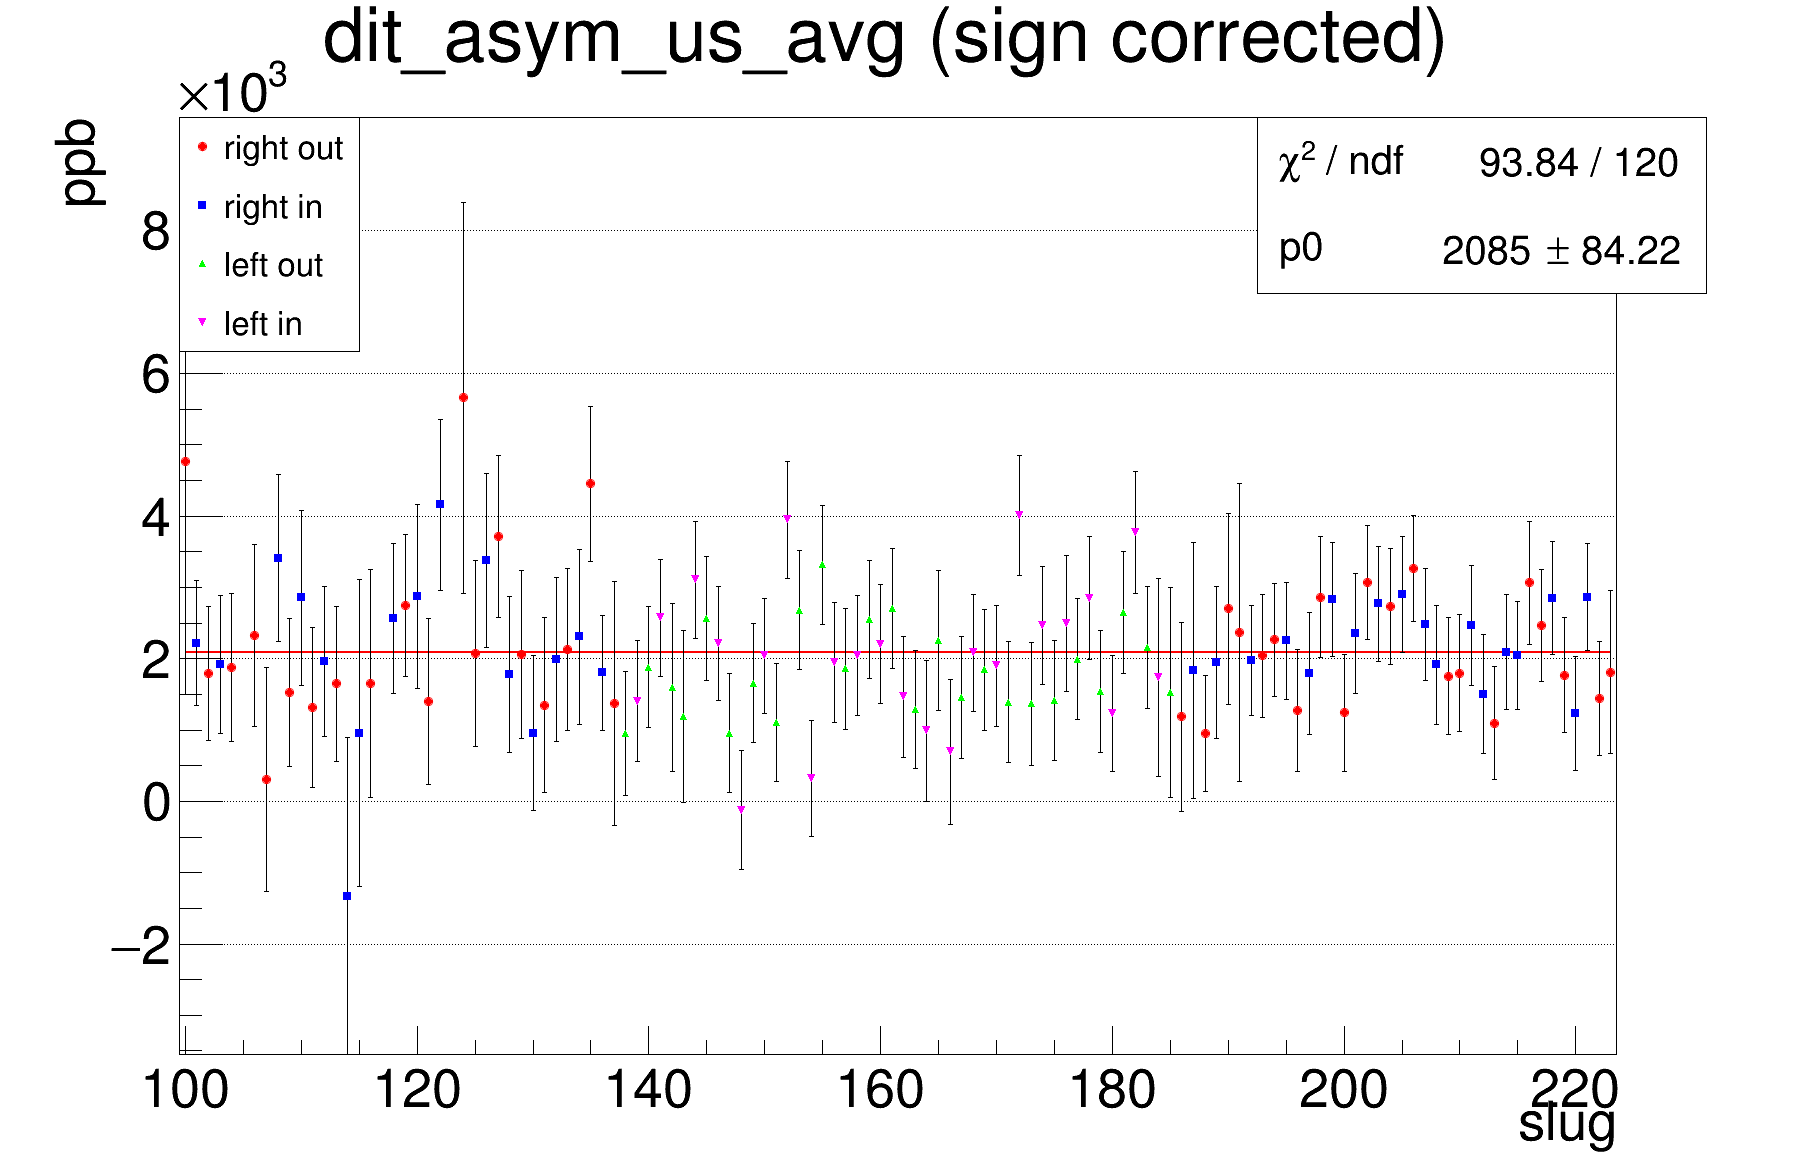
\includegraphics[width=0.49\linewidth]{crex_dit_asym_us_avg}
    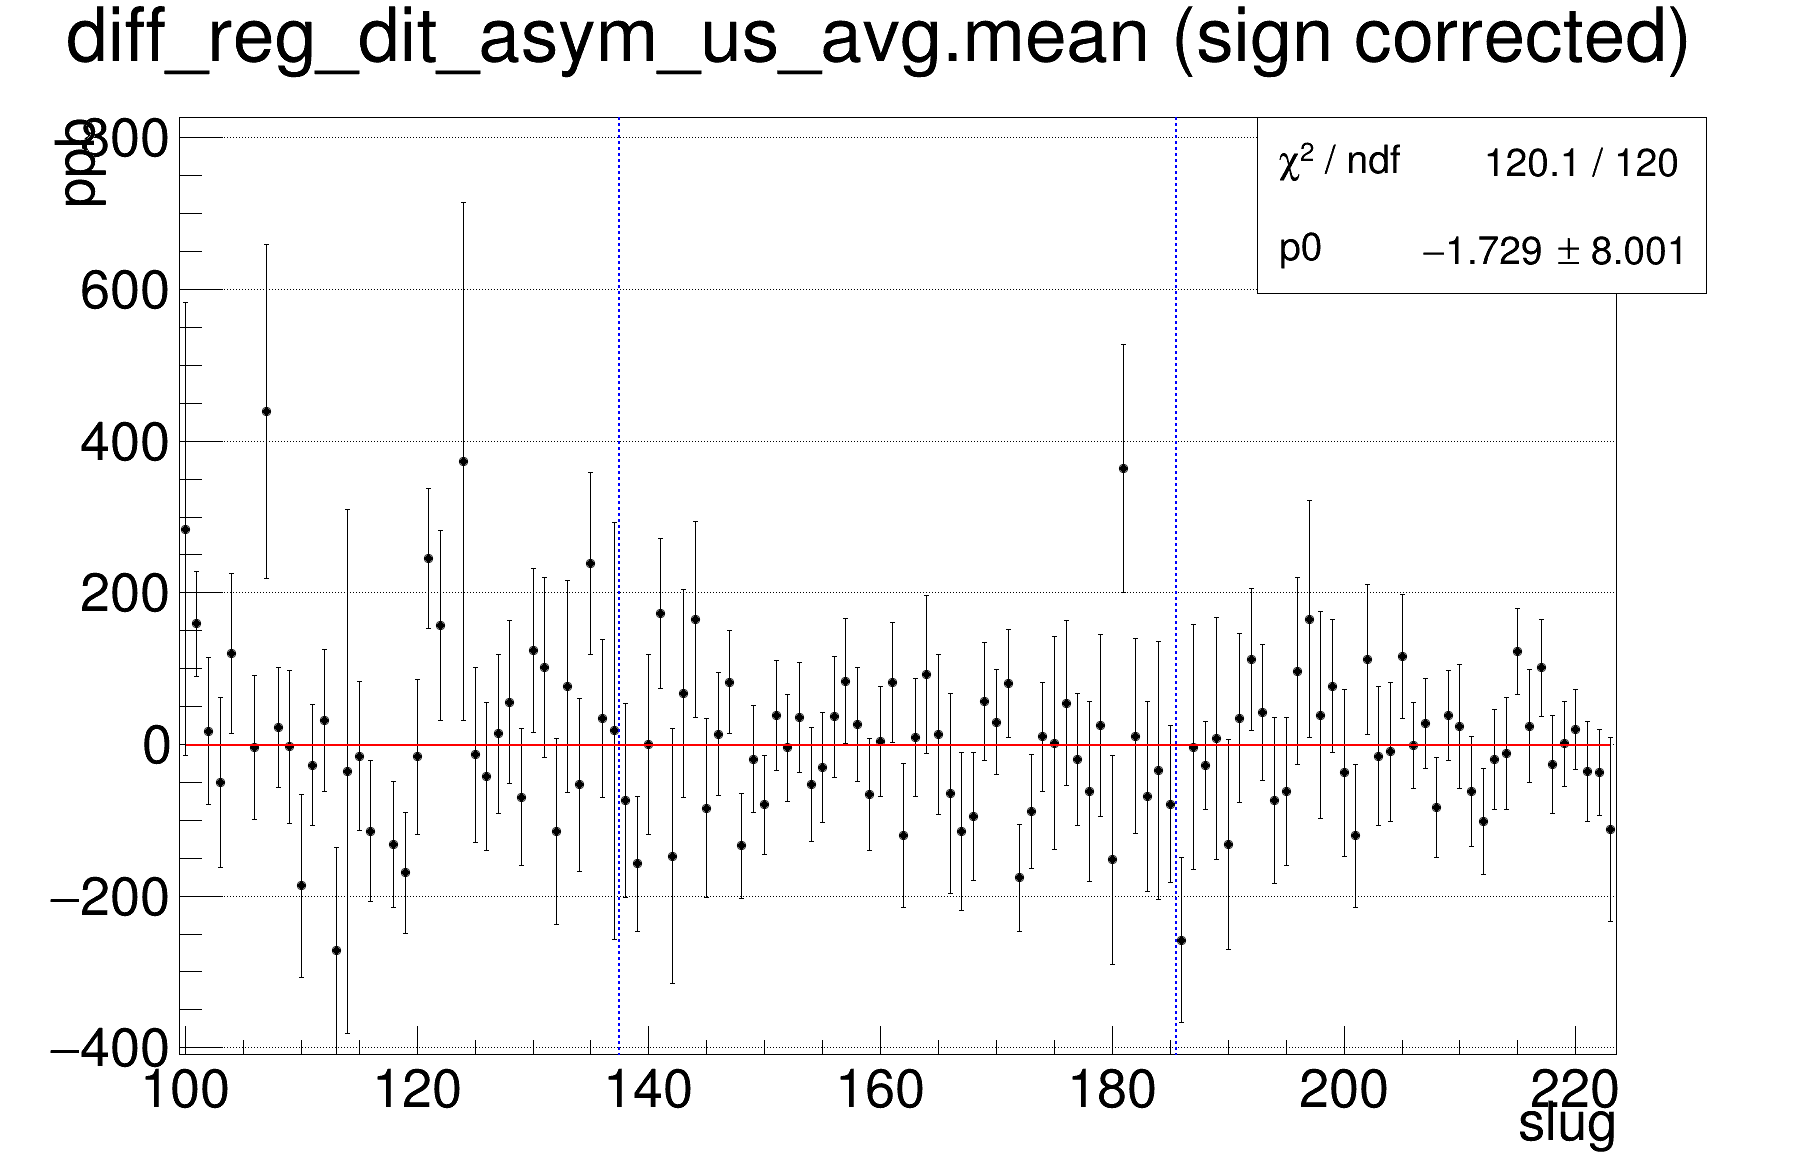
\includegraphics[width=0.49\linewidth]{crex_diff_reg_dit_asym_us_avg.mean}
    \caption[Dithering corrected asymmetry]
    {Left: slug-wise scatter plot of the asymmetry corrected with beam modulation.
    Right: difference between the asymmetry values corrected by regression and
    beam modulation.}
    \label{fig:dit_result}
\end{figure}


%%%%%%%%%%%%%%%%%%%%%%%%%%%%%%%%%%%%%%%%%%%%%%%%
\subsection{Lagrange Multiplier}
As mentioned earlier, we should use miniruns for a more precise false asymmetry correction.
However, in the dithering correction, segment-wise slopes are used due to the limited
availability of modulation data. While the regression method is more precise than the dithering correction, it is less accurate due to the inherent noise present in detectors and monitors.
The modulation amplitude is designed to be larger than the noise level (while still being small compared to the yield, typically less than 1\%). This design allows for increased accuracy by effectively suppressing the impact of those noises.

Considering the strengths and weaknesses of both methods, it is natural to 
explore a combination that leverages their respective advantages. This integration
leads to the Lagrangian analysis, which is actually regression with constraints from beam modulation.

From Eq.~\ref{eq:regression_chi2}, the $\chi^2$ for the asymmetry regression is
derived as:
\begin{equation}
    \chi^2 = \sum_i \left( \CA_{\text{raw}} - \sum_\mu \beta_\mu \Delta M_\mu \right)_i^2
\end{equation}
where i sums over samples and $\mu$ iterates over selected BPMs.

The Lagrangian multiplier for this constraint problem will be:
\begin{equation}
    \CL = \sum_i \left( \CA_{\text{raw}} - \sum_\mu \beta_\mu \Delta M_\mu \right)_i^2+ \sum_\alpha \lambda_\alpha \left(\sum_\mu \beta_\mu \frac{\partial M_\mu}{\partial C_\alpha} - \frac{\partial D}{\partial C_\alpha} \right)
\end{equation}
$\alpha$ indexes the selected coils.

Set the gradient of $\CL$ to zero:
\begin{equation}
    \begin{aligned}
	\frac{\partial \CL}{\partial \beta_\mu} 
	&= -2\Delta M_\mu \sum_i \left( \CA_{\text{raw}} 
	  - \sum_\nu \beta_\nu \Delta M_\nu \right)_i + \sum_\alpha \lambda_\alpha \frac{\partial M_\mu}{\partial C_\alpha}    \\
	&= 2 \left(\sum_\nu \beta_\nu \cdot \text{cov}(\Delta M_\mu, \Delta M_\nu) 
	  - \text{cov}(\CA_{\text{raw}}, \Delta M_\mu) \right) + \sum_\alpha \lambda_\alpha \frac{\partial M_\mu}{\partial C_\alpha} = 0  \\
	\frac{\partial \CL}{\partial \lambda_\alpha} &= \left( \sum_\mu \beta_\mu \frac{\partial M_\mu}{\partial C_\alpha} - \frac{\partial D}{\partial C_\alpha} \right) = 0\\
    \end{aligned}
    \label{eq:lagrange_derivative}
\end{equation}

The distinction between the second formula of Eq.~\ref{eq:lagrange_derivative} and
the conventional beam modulation method may be confusing, because they are actually
the same if we consider only five BPMs. The beam modulation constraint is so 
strong that it directly determines the slope values. However, as we introduce
more BPMs into the analysis, surpassing the number of coils, the solution
to the constraint becomes non-unique. Consequently, the Lagrange multiplier
method becomes applicable.

Write Eq.~\ref{eq:lagrange_derivative} in a matrix form:
\begin{equation}
    \begin{pmatrix}
	M_{m\times m}	& (B^T)_{m\times n}	\\
	B_{n \times m}  & \bm{0}_{n\times n}   \\
    \end{pmatrix}
    \begin{pmatrix}
	\beta_1	\\
	\vdots	\\
	\beta_m	\\
	\frac{\lambda_1}{2} \\
	\vdots	\\
	\frac{\lambda_n}{2} \\
    \end{pmatrix}
    =
    \begin{pmatrix}
	\text{cov}(\CA_{raw}, \Delta M_1)  \\
	\vdots	\\
	\text{cov}(\CA_{raw}, \Delta M_m)  \\
	\frac{\partial D}{\partial C_1}	\\
	\vdots	\\
	\frac{\partial D}{\partial C_n}	\\
    \end{pmatrix}
    \label{eq:lagrange_derivative_1}
\end{equation}
where the $M$ and $B$ matrices are defined in Eq.~\ref{eq:M_definition} and \ref{eq:B_definition},
and $m$ ($n$) refers to the number of BPMs (coils) with $m > n$.
In our analysis, we used all 12 BPMs, so $m = 12$ and $n = 5$.

Eq.~\ref{eq:lagrange_derivative_1} can be solved to be
\begin{equation}
    \begin{pmatrix}
	\vec{\beta} \\
	\vec{\lambda}	\\
    \end{pmatrix}
    =
    \begin{pmatrix}
	M   & B^T   \\
	B   & \bm{0}	\\
    \end{pmatrix}^{-1}
    \times
    \begin{pmatrix}
	\vec{Y}_1   \\
	\vec{Y}_2   \\
    \end{pmatrix}
\end{equation}
where $\vec{\beta}$ and $\vec{\lambda}$ are the slope vector and the Lagrange multiplier vector,
$\vec{Y}_1$ is the covariance between raw asymmetry and monitor difference, 
and $\vec{Y}_2$ is the detector sensitivity. As what we did in the beam modulation, 
the sensitivity values are segment-wise average values.

% The difference between the Lagrange multiplier and regression
\subsubsection{Lagrange Multiplier Result}
The asymmetry corrected with the Lagrange multiplier is shown in 
Fig.~\ref{fig:crex_corrected_asym}. Compared with the asymmetry values corrected
using the other two methods, only a tiny difference is observed.
\begin{figure}[!h]
    \centering
    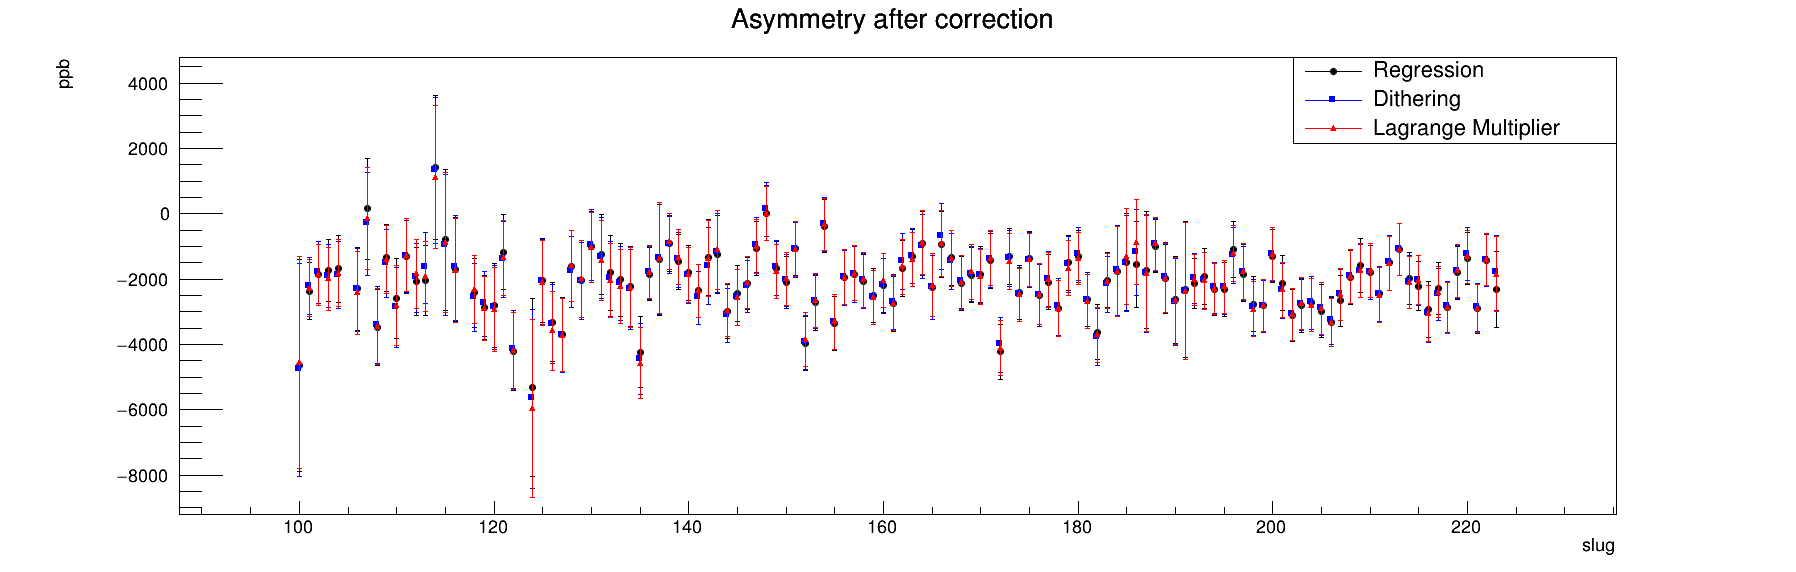
\includegraphics[width=\linewidth]{crex_corrected_asym}
    \caption{Comparison of the asymmetry values corrected using regression (black), 
    dithering (blue) and the Lagrange multiplier (red).}
    \label{fig:crex_corrected_asym}
\end{figure}

%%%%%%%%%%%%%%%%%%%%%%%%%%%%%%%%%%%%%%%%%%%%%%%%%%%%%%%%%%%%%%%%%%%%%%%%
\section{Result}
As discussed before, the slow helicity reversal involving the IHWP and the 
double Wien filters, allow us to investigate potential systematic biases. 
In this context, define a `part' as a set of sharing the same IHWP and Wien-flip states.
By examining the part asymmetry presented in Fig.~\ref{fig:crex_part_pitt}, 
it is evident that the measured asymmetries with opposite IHWP states 
or opposite Wien-flip states overlap within a $1\sigma$ uncertainty range. 
This observation verifies the unbiasedness of our measurement.

% pitt: https://docs.google.com/spreadsheets/d/1LdoBsa34J5YpNRZqGgA_A9wKwgx2oydEu621Fswt75c/edit#gid=862711716
The pitt plot in Fig.~\ref{fig:crex_part_pitt} shows the asymmetry distribution
for each pitt. The concept of pitt was introduced by Mark Pitt and involves grouping
nearby slugs with alternating IHWP states in order to achieve a comparable number of events for opposite IHWP states within each pitt.
Typically, each pitt consists of about 4 slugs, the detailed range definition
of each pitt can be found in Cameron's thesis.

%%%%%%%%%%%%%%%%%%%%%%%%
\subsubsection{The Final Number}
\begin{figure}
    % comparison of asymmetry from largest time scale to smallest time scale:
    % Wien, pitt, slug, run
    \centering
    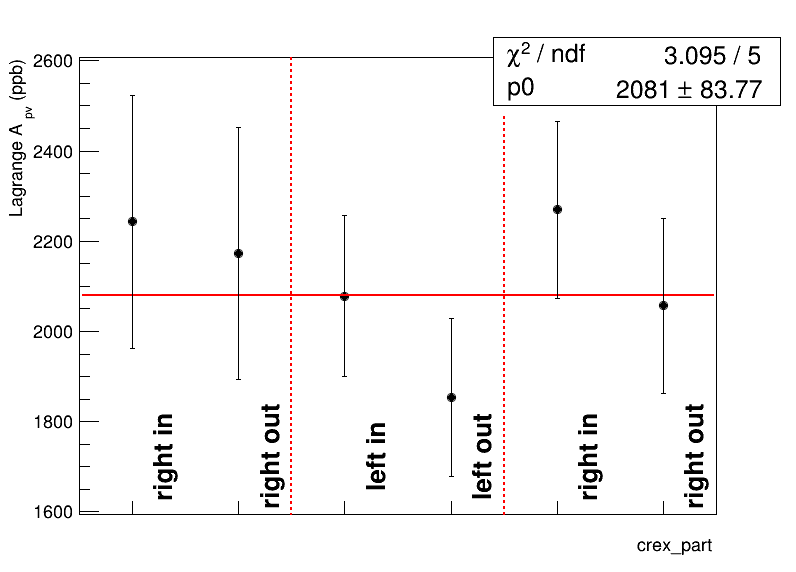
\includegraphics[width=0.49\linewidth]{crex_part_eigen_lagr_asym_main_det_1}
    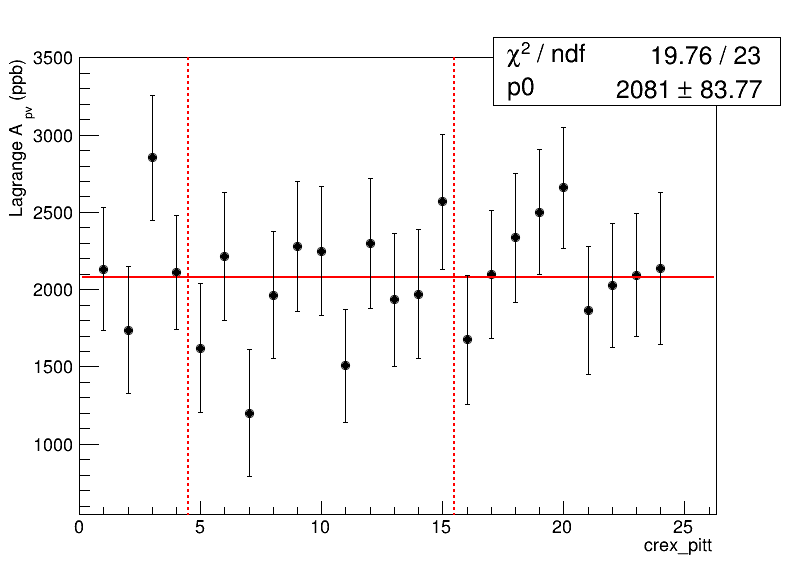
\includegraphics[width=0.49\linewidth]{crex_pitt_eigen_lagr_asym_main_det_1}
    \caption{Part-wise and pitt-wise scattering plot of asymmetry values
    corrected with the Lagrange multiplier.}
    \label{fig:crex_part_pitt}
\end{figure}

From the pitt plot in Fig.~\ref{fig:crex_part_pitt}, 
the final corrected asymmetry (blinded) is read as: 
\begin{equation}
    \CA_{\text{cor}} = 2081 \pm 83.77\ \mathrm{ppb}
\end{equation}
The number used in the published paper is
\begin{equation}
    \CA_{\text{cor}} = 2080 \pm 83.77\ \mathrm{ppb}
\end{equation}
The difference lies in the 2 miniruns I discard in Table~\ref{tab:short_miniruns} because of their small
sample sizes.
